% Dokumentklassen:
% article, report, beamer, book, letter etc.
% https://en.wikibooks.org/wiki/LaTeX/Document_Structure
\documentclass[a4paper]{article}

% Seitenränder Abstand setzen
\usepackage[margin=80pt]{geometry}

% Deutsches Sprachpaket
\usepackage[english]{babel}
% UTF8 Input Encoding
\usepackage[utf8]{inputenc}

\usepackage{amsmath}
\usepackage{amssymb}

% Schriftbild ändern
% https://en.wikibooks.org/wiki/LaTeX/Fonts
\usepackage[scaled]{helvet}
% (Sans) Serifen oder anderes
% \rmdefault: Serifen
% \sfdefault: Sans-Serifen
% \ttdefault: Typewriter
\renewcommand{\familydefault}{\sfdefault}
% Fontencoding (für ä, ö, ü etc.)
\usepackage[T1]{fontenc}

% Gänsefüsschen richtig kompilieren
\usepackage [autostyle]{csquotes}
\MakeOuterQuote{"}

% Hyperlinks farblos
\usepackage[hidelinks]{hyperref}
\hypersetup{colorlinks=false}

% Package für Aufzählungen
\usepackage{enumitem}
% kein Abstand zwischen Aufzählungen
% Sollen doch Abstände vorhanden sein: nach Aufzählung {itemsep=1em}
\setlist{nosep}

% Grafik-Packages, für Figures, Subfigures und PDF als Import
\usepackage{graphicx}
\usepackage{subcaption}
\usepackage{pdfpages}

% Package und Einstellungen für Java-Code-Darstellung
% Werden erstellt mit \begin{lstlisting}
\usepackage{listings}
\usepackage{color}
\definecolor{dkgreen}{rgb}{0,0.6,0}
\definecolor{gray}{rgb}{0.5,0.5,0.5}
\definecolor{mauve}{rgb}{0.58,0,0.82}
\lstset{ %
	language=R,                     % the language of the code
	basicstyle=\footnotesize,       % the size of the fonts that are used for the code
	numbers=left,                   % where to put the line-numbers
	numberstyle=\tiny\color{gray},  % the style that is used for the line-numbers
	stepnumber=1,                   % the step between two line-numbers. If it's 1, each line
	% will be numbered
	numbersep=5pt,                  % how far the line-numbers are from the code
	backgroundcolor=\color{white},  % choose the background color. You must add \usepackage{color}
	showspaces=false,               % show spaces adding particular underscores
	showstringspaces=false,         % underline spaces within strings
	showtabs=false,                 % show tabs within strings adding particular underscores
	frame=single,                   % adds a frame around the code
	rulecolor=\color{black},        % if not set, the frame-color may be changed on line-breaks within not-black text (e.g. commens (green here))
	tabsize=2,                      % sets default tabsize to 2 spaces
	captionpos=b,                   % sets the caption-position to bottom
	breaklines=true,                % sets automatic line breaking
	breakatwhitespace=false,        % sets if automatic breaks should only happen at whitespace
	title=\lstname,                 % show the filename of files included with \lstinputlisting;
	% also try caption instead of title
	keywordstyle=\color{blue},      % keyword style
	commentstyle=\color{dkgreen},   % comment style
	stringstyle=\color{mauve},      % string literal style
	escapeinside={\%*}{*)},         % if you want to add a comment within your code
	morekeywords={*,...}            % if you want to add more keywords to the set
} 

\title{\textbf{Module Summary DASB - Slides} \\
Data Science Basics}
\date{\today}
\author{Maurin D. Thalmann}

\begin{document}
	
	\pagenumbering{gobble}
	\maketitle
	
	\newpage
	\pagenumbering{arabic}
	\tableofcontents
	
	\newpage
	
	\section{Learning Objectives}
	
		\paragraph{Introduction to Data Science}
		
			\begin{itemize}
				\item Define the term "Data Science" and differentiate it from similar concepts such as big data, data mining, OLAP, predictive modeling, data analysis
				\item Describe why and how value is created from data, especially in form of processes
				\item Describe the skills and activities of a data science professional
				\item Describe possible applications of data science
			\end{itemize}
		
		\paragraph{Intro to R and Exploratory Data Analysis (EDA)}
		
			\begin{itemize}
				\item Define the term "Exploratory Data Analysis" and explain why it is a fundamental part of making data science
				\item Give a short introduction to R and present its main features
				\item Indicate the key actors and actions that compose EDA and how they are related to the data sources considered
				\item Indicate different ways of importing data into R for analysis and how to check for their quality
				\item Describe the main operations available in R (through libraries) to manipulate data and prepare it for the analysis
			\end{itemize}
		
		\paragraph{ggplot2 and its usage in EDA}
		
			\begin{itemize}
				\item Define the role of graphical representations in the "Exploratory Data Analysis" and explain why it is a fundamental tool to make it effective
				\item Give a short introduction to ggplot2 and its features
				\item Ddescribe the main way of working of ggplot2 and how to compose complex graphs (e.g.: representing more than 3 variables in a single graph, for multidimensional data)
				\item Explain the role of the facets and how they can support the representation of "partial" relationships
				\item Indicate the role of the coordinates in the graph usage for EDA
			\end{itemize}
		
		\paragraph{Intro to Forecasting}
		
			\begin{itemize}
				\item Understand and explain the concept of forecasting
				\item Present the basic approach, either using the theory or by example
				\item Present a linear model and describe its basic characteristics
				\item Indicate how EDA can support and scaffold the model identification
				\item Apply basic forecasting in R, given the datasource
			\end{itemize}
		
		\paragraph{Forecasting Models: Usage / Application}
		
			\begin{itemize}
				\item Presents the limits of the linear models
				\item Define the way of extending linear models
				\item Justify forecasting \& interpretation (phenomena comprehension) in data science, also by presenting examples
				\item Present advantages and limits of the defined extensions
				\item Presenting Parametric and Nonparametric idea in model definition (ML)
				\item Indicate how EDA can support and scaffold the model identification
				\item Apply more advanced forecasting in R, given the datasource
			\end{itemize}
		
		\paragraph{Ethics in Data Science}
		
			\begin{itemize}
				\item List ethical issues with big data analytics
				\item Know the conditions for processing of personal data
				\item Know the Rights of Individuals regarding personal data processing
				\item Provide recommendations for more ethical data science
				\item Being able to analyze a given case and provide conclusion on the ethical aspects involved
			\end{itemize}
		
	\newpage
	
	\section{Introduction to Data Science}
	
		\subsection{Introductory Stizzle}
		
		\begin{itemize}
			\item More is different - with different quantity comes different quality, although "more" is always dependent on the point of view.
			\item Data volume nowadays is exploding (276.12 billion GB of digital data)
			\item Data Science tries to close the gap between "Data \textit{available} to an organization" and "Percent of data an organization can \textit{process}".
		\end{itemize}
	
		\begin{figure}[htb!]
			\centering
			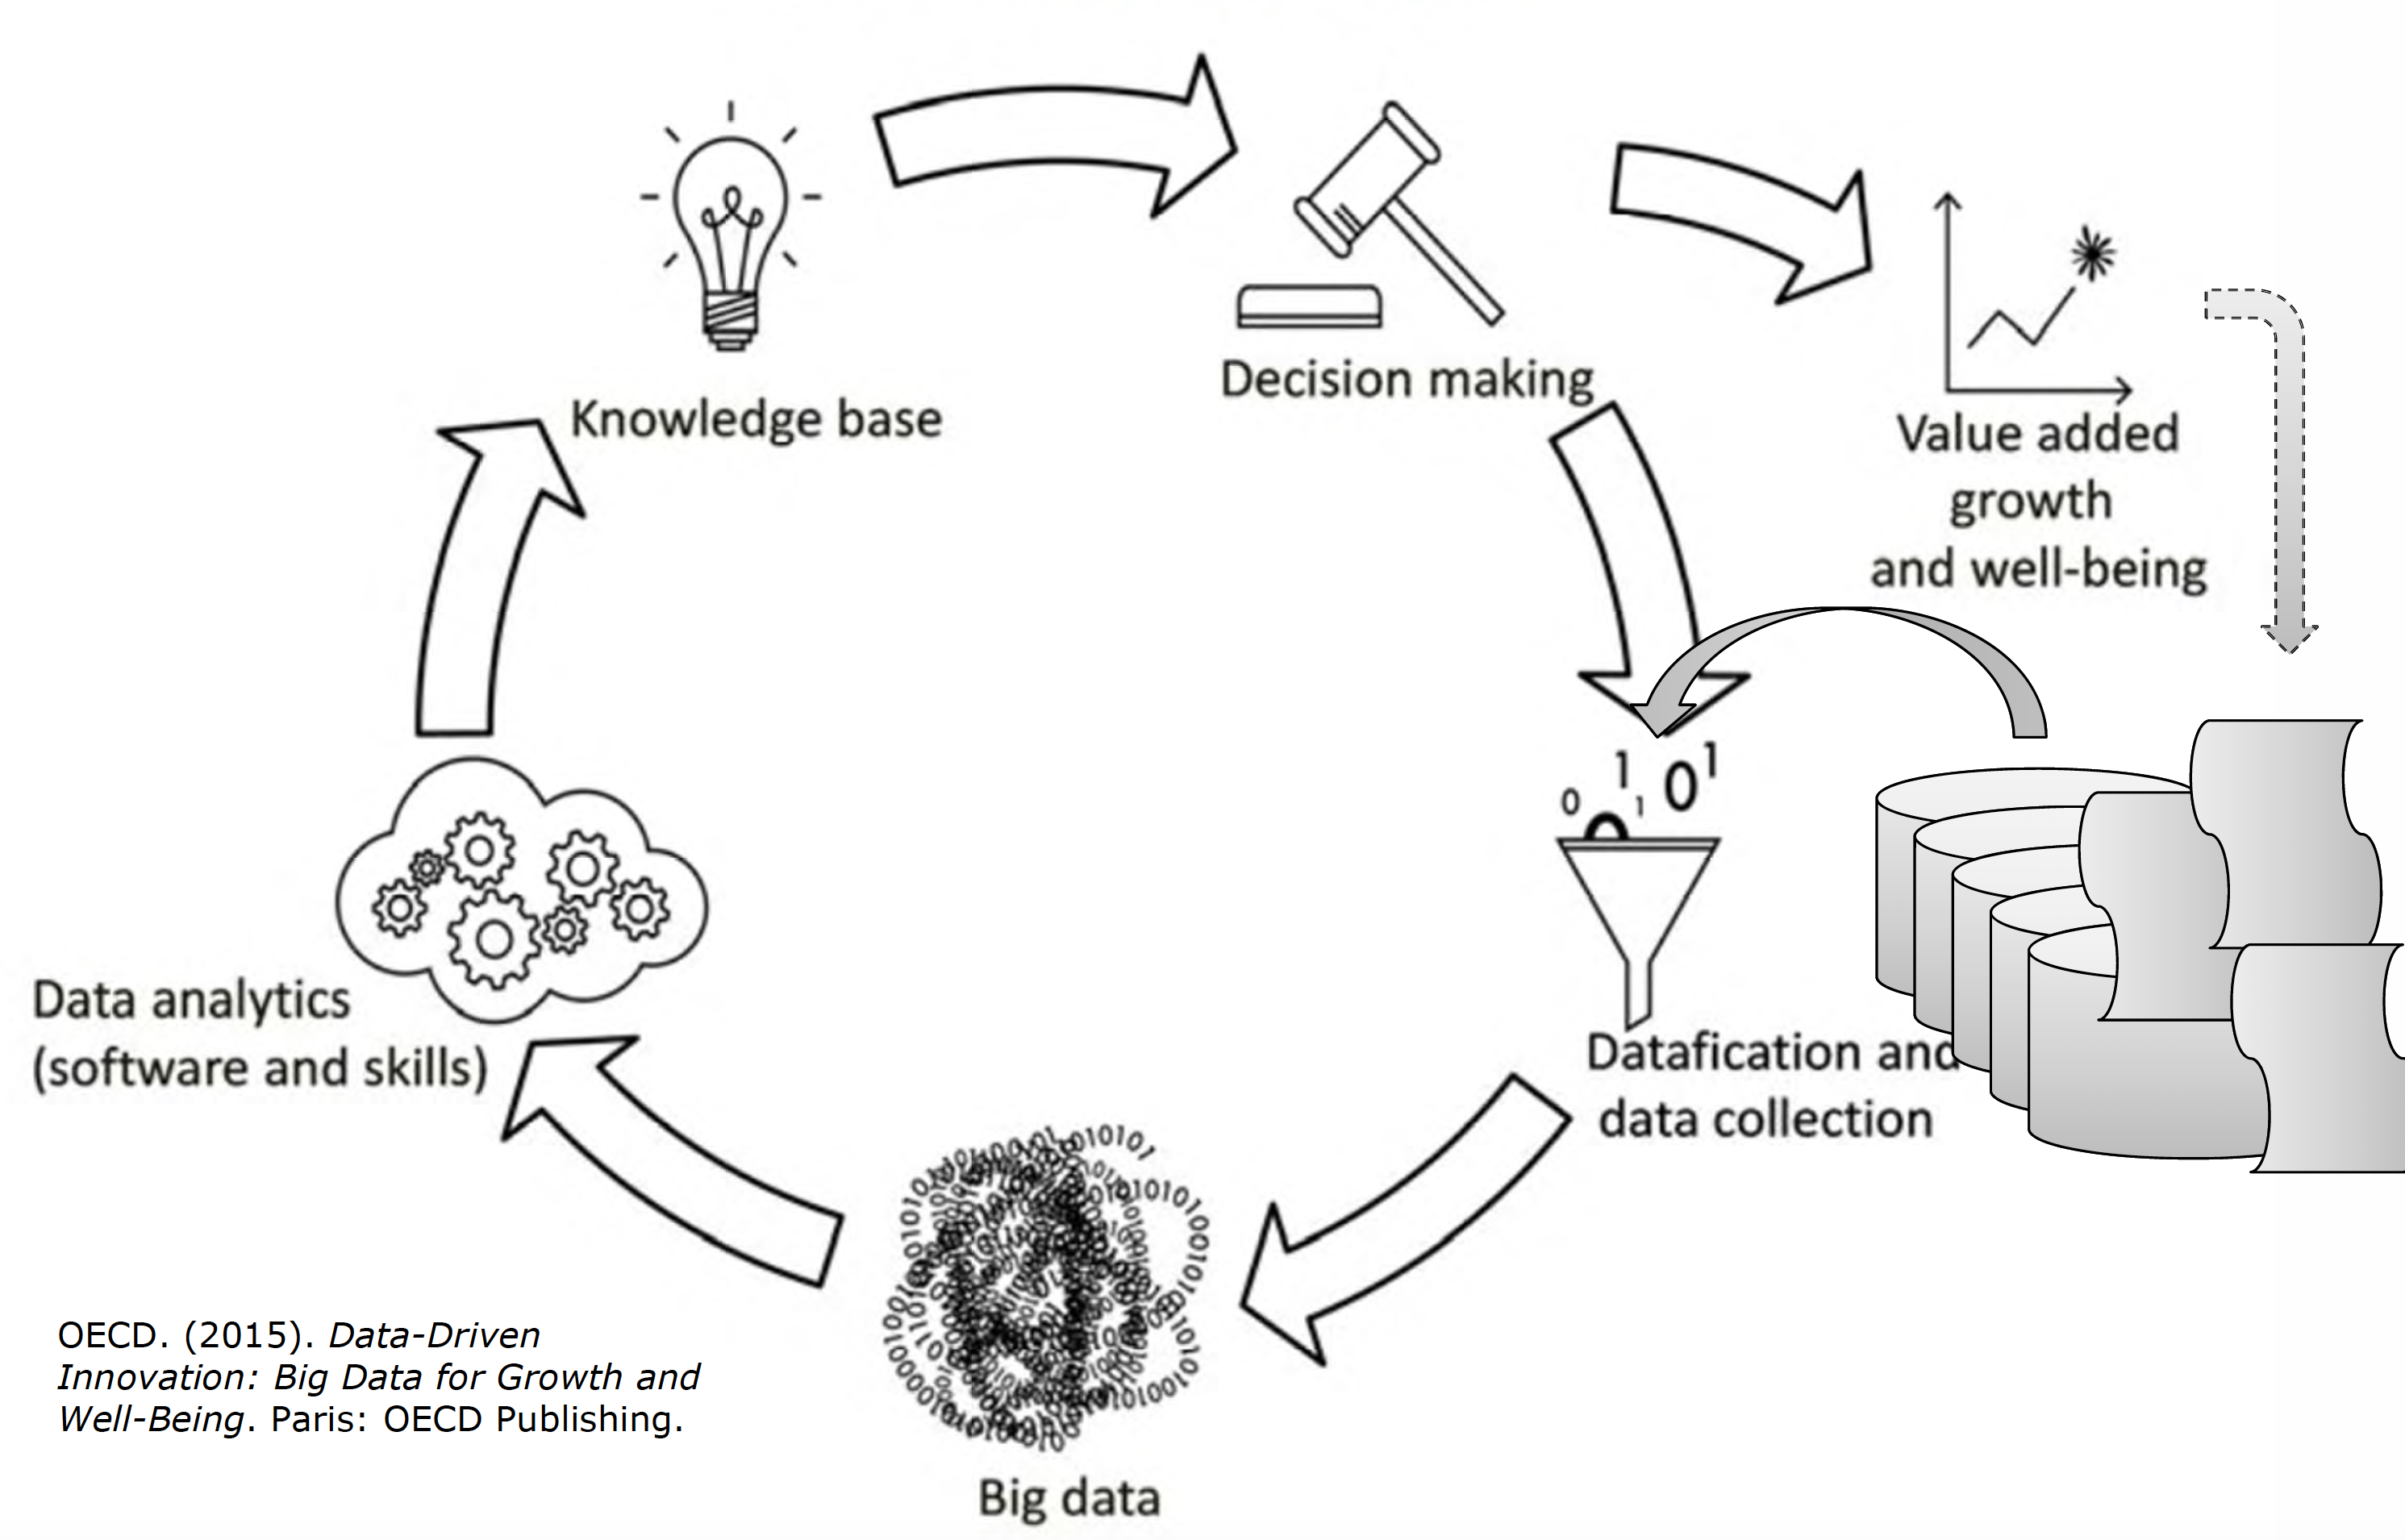
\includegraphics[width=0.5\textwidth]{img/sw01/data_value_cycle.png}
			\caption{Beautiful illustration of the classic data value cycle}
		\end{figure}
	\noindent
		"\textbf{Data Science} is the extraction of actionable knowledge directly from data through a discovery, or hypothesis formulation and hypothesis testing".
		Data Scientists generate knowledge from big data.
		
		\begin{figure}[htb!]
			\centering
			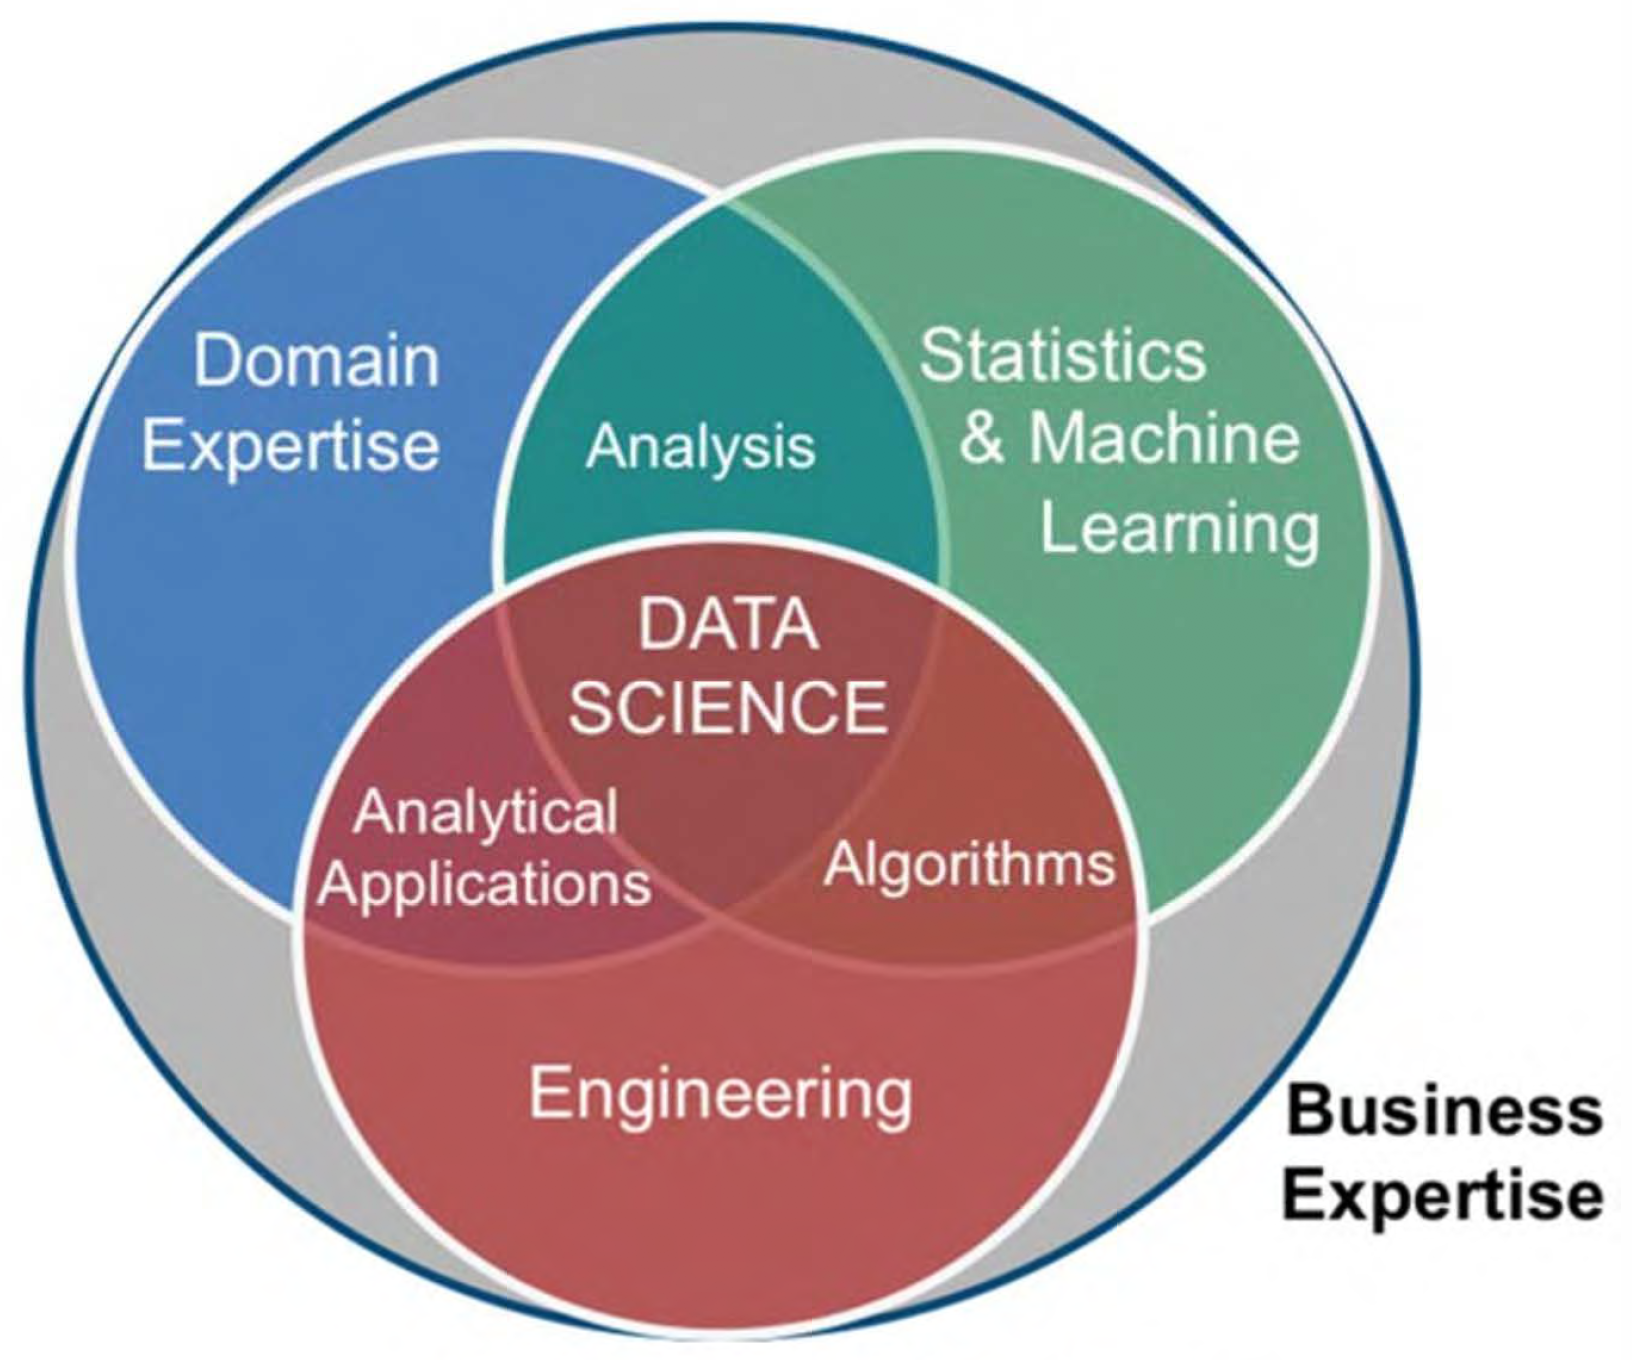
\includegraphics[width=0.3\textwidth]{img/sw01/ds_skills.png}
			\caption{Skills needed in Data Science}
		\end{figure}
	
		\subsection{A Global View on Data Science}
		
		\begin{figure}[htb!]
			\centering
			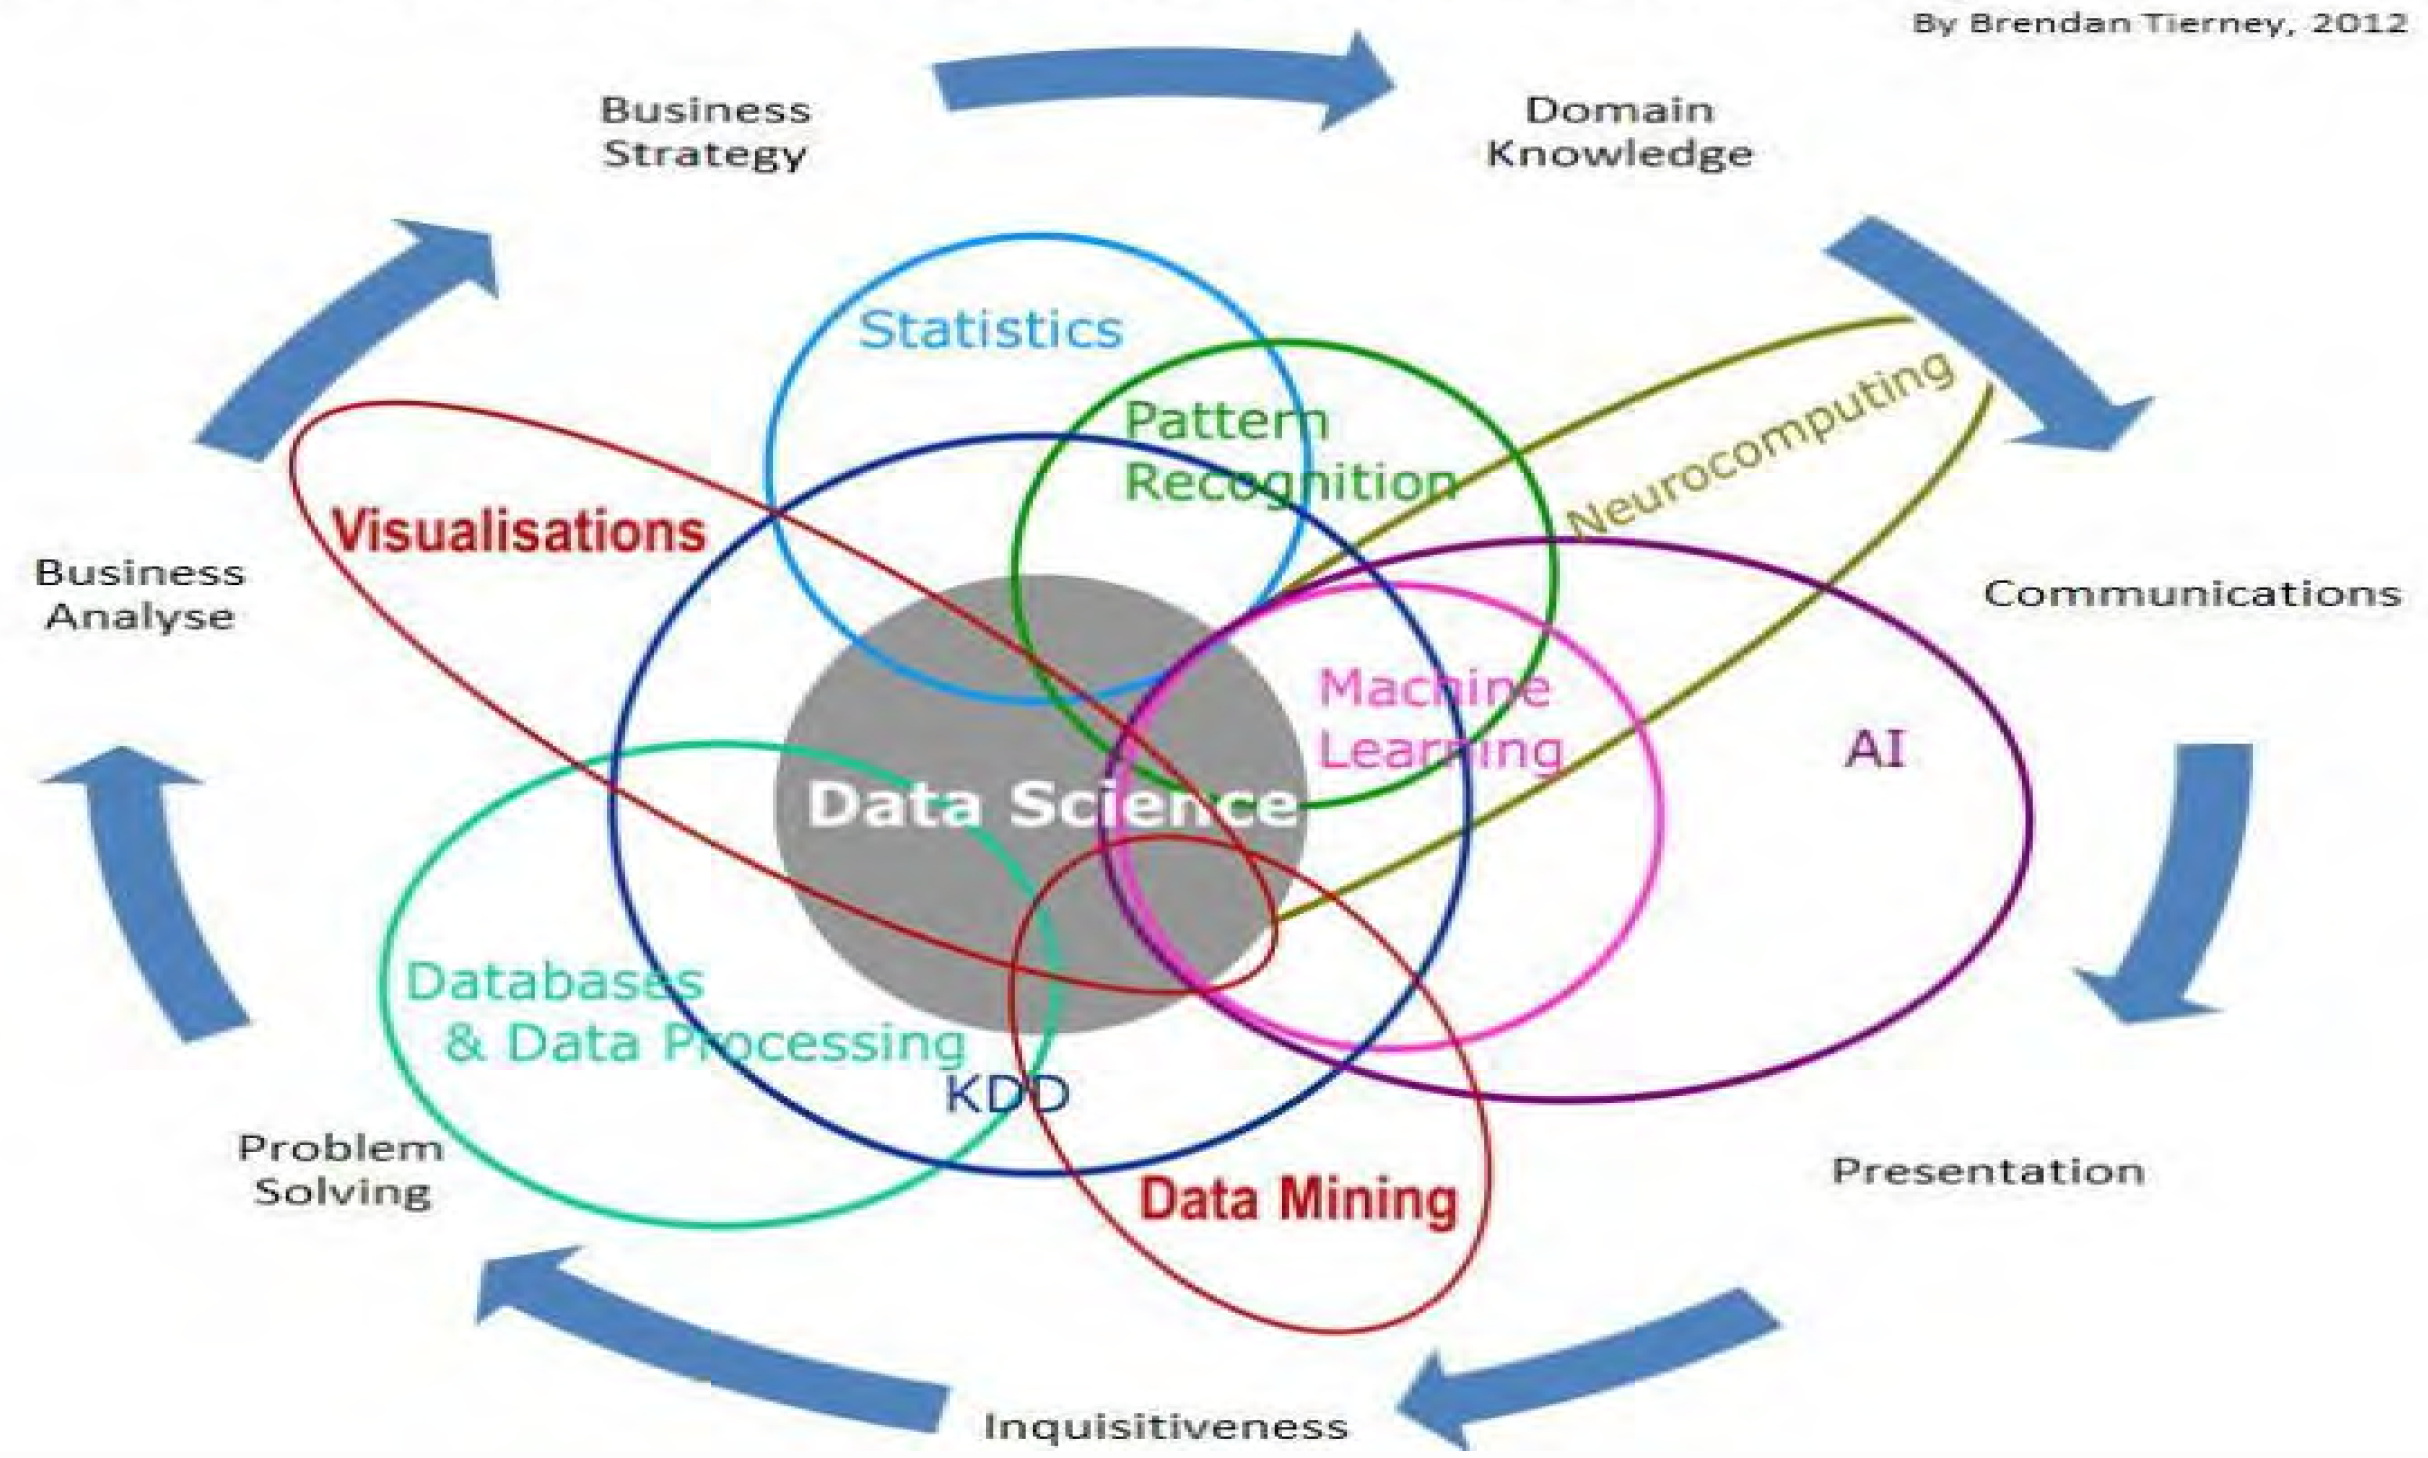
\includegraphics[width=0.5\textwidth]{img/sw01/multidisc.png}
			\caption{Data Science is multidisciplinary}
		\end{figure}
	
		\newpage
		
		\begin{itemize}
			\item \textbf{AI}: programs that perform tasks resembling humans (learn and reason)
			\item \textbf{ML}: algorithms to learn from that data without explicit programming
			\item \textbf{DL}: subset of ML using artificial neural networks for treating vast amount of data (big data)
			\item \textbf{Data Science}: spans the collection, management, analysis and interpretation of large amounts of data with a wide range of applications $\rightarrow$
				make informed decisions based on what was learned
			\item \textbf{EDA} (exploratory data analysis): extract insight from data (outside AI, human based)
		\end{itemize}
	
		\begin{figure}[htb!]
			\centering
			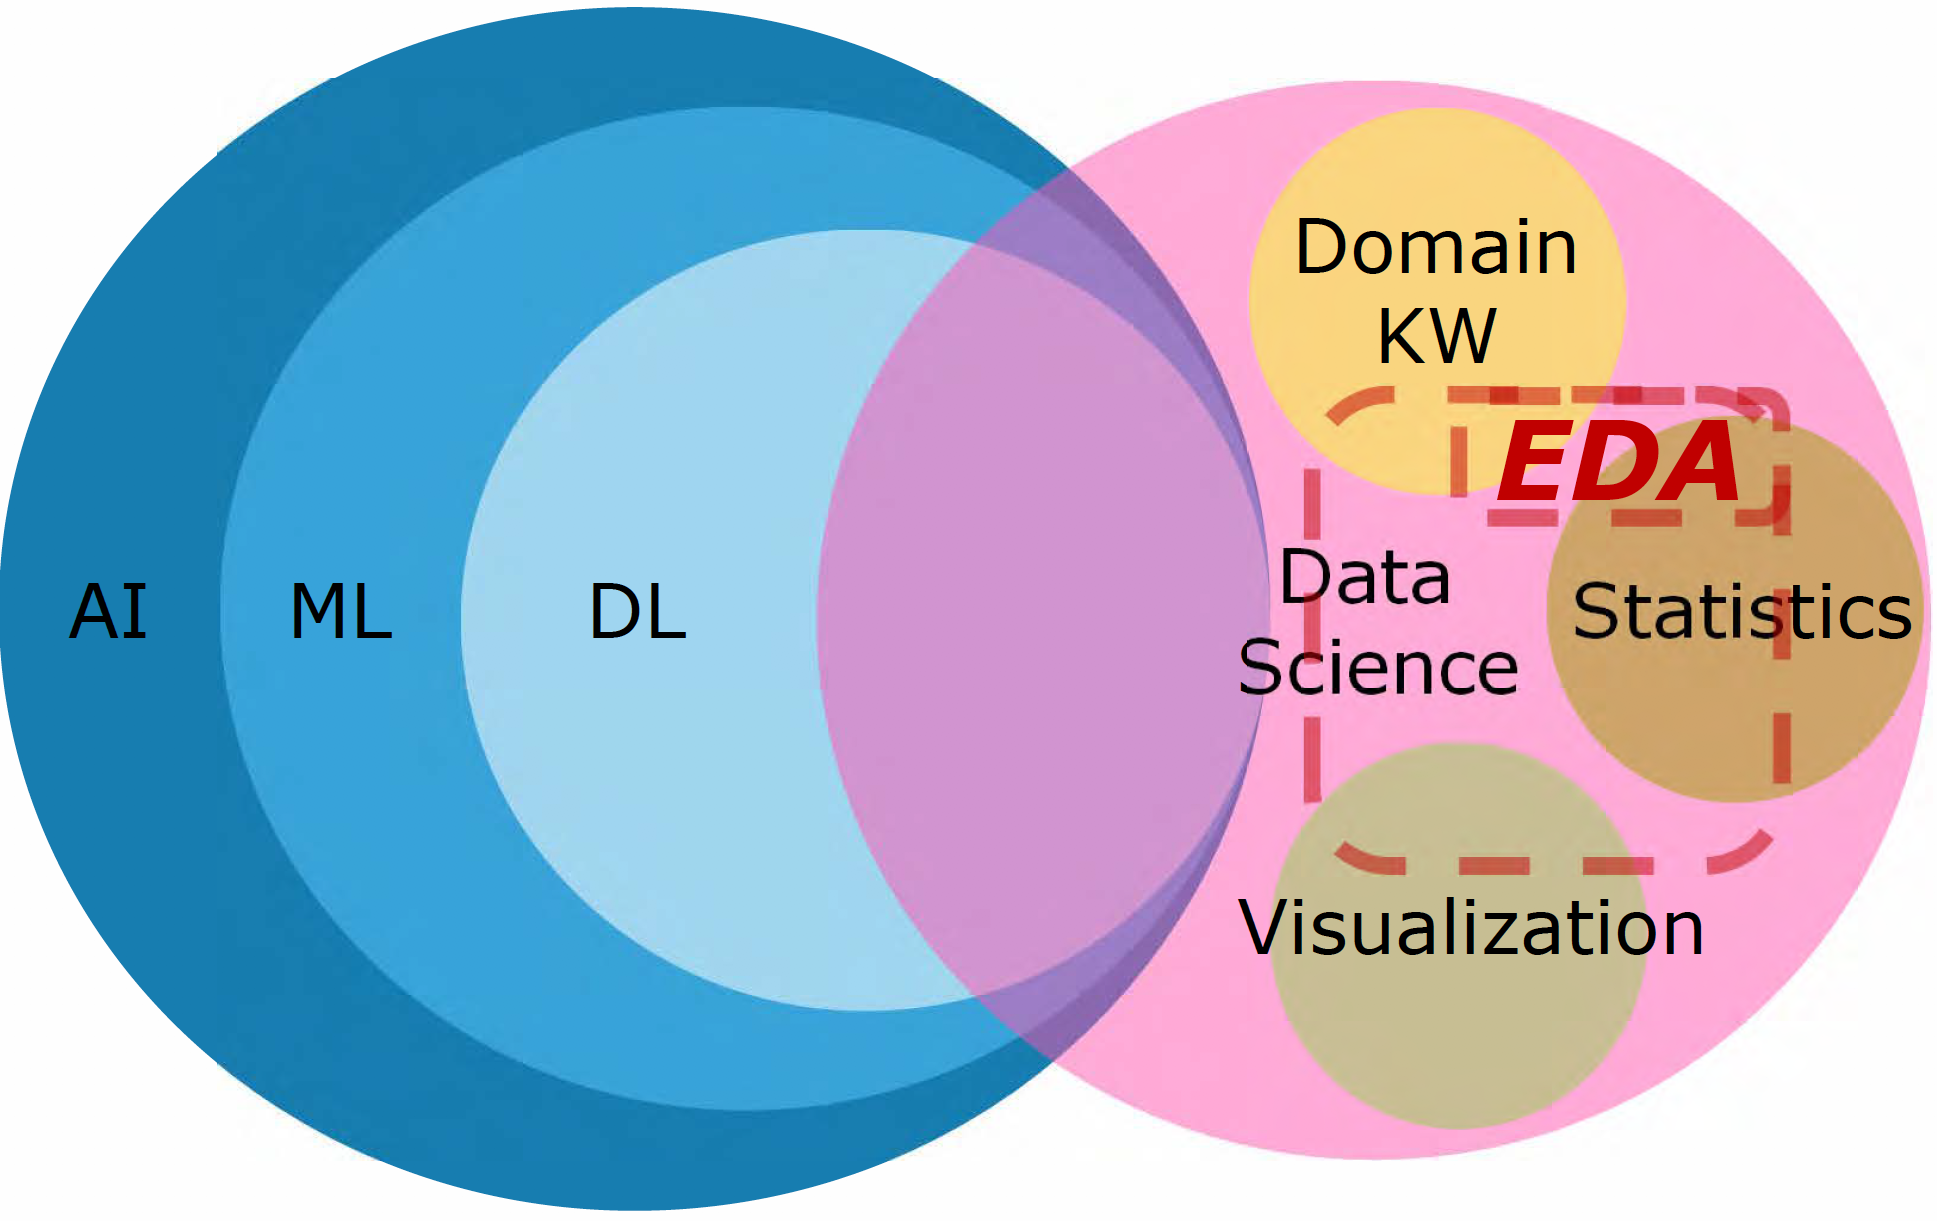
\includegraphics[width=0.4\textwidth]{img/sw01/global_view.png}
			\caption{AI / ML / DL and Data Science}
		\end{figure}
	
		\subsection{Different Concepts in Data Analytics}
		
			\subsubsection{1993 - Online Analytical Processing (OLAP)}
			
			\begin{minipage}[c]{0.3\textwidth}
				\centering
				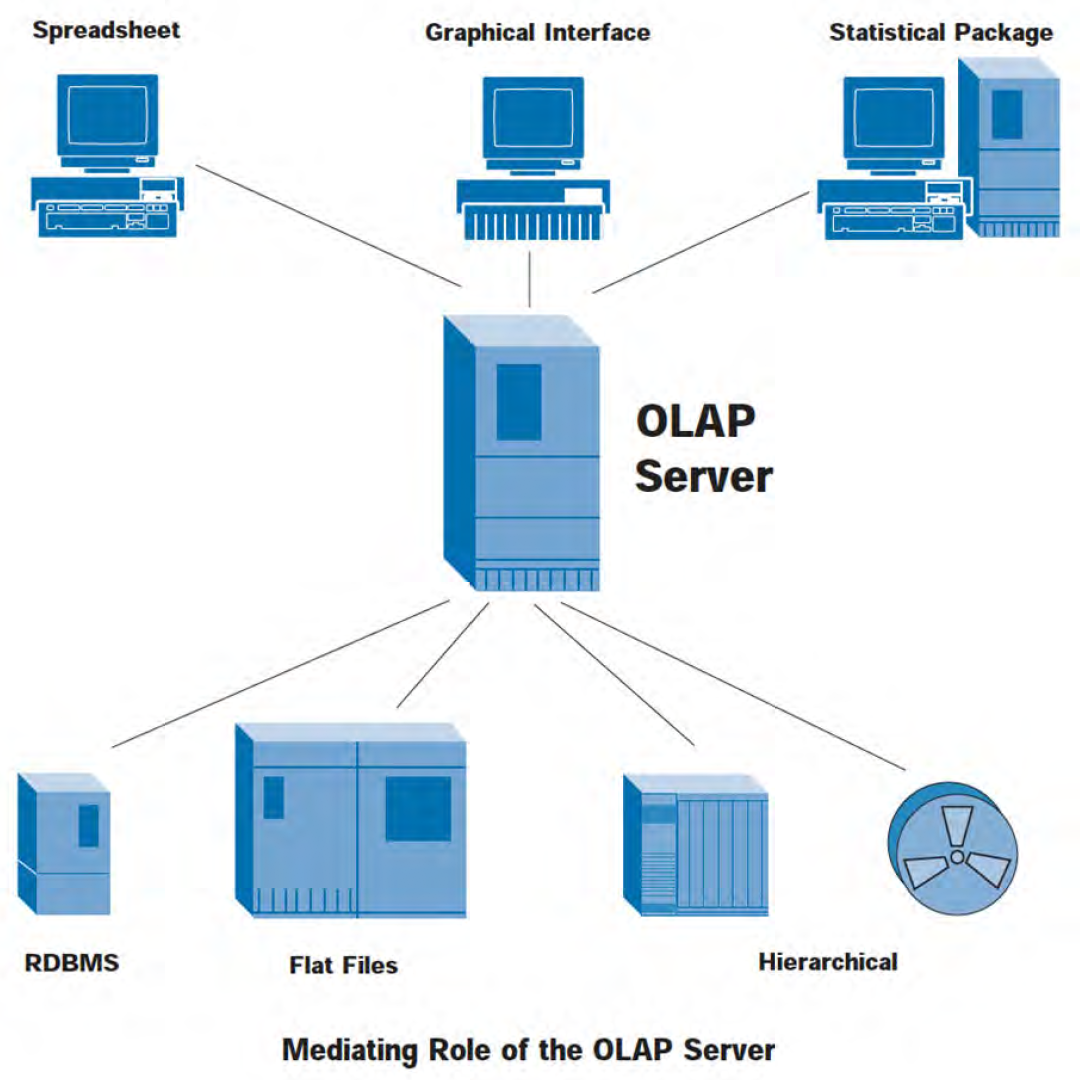
\includegraphics[width=\textwidth]{img/sw01/olap.png}
			\end{minipage}
			\hfill
			\begin{minipage}[c]{0.6\textwidth}
				\begin{itemize}
					\item It's online, not batch (interactive, not programmed in COBOL)
					\item The OLAP system should access the data required to perform the indicated analysis
					\item OLAP tools empower useranalysts to earily perform multi-dimensional analysis, which previously have been avoided because of their perceived complexity.
				\end{itemize}
			\end{minipage}
		
			\subsubsection{1998 - Fuzzy Data Analysis}
			
			\begin{minipage}[c]{0.3\textwidth}
				\centering
				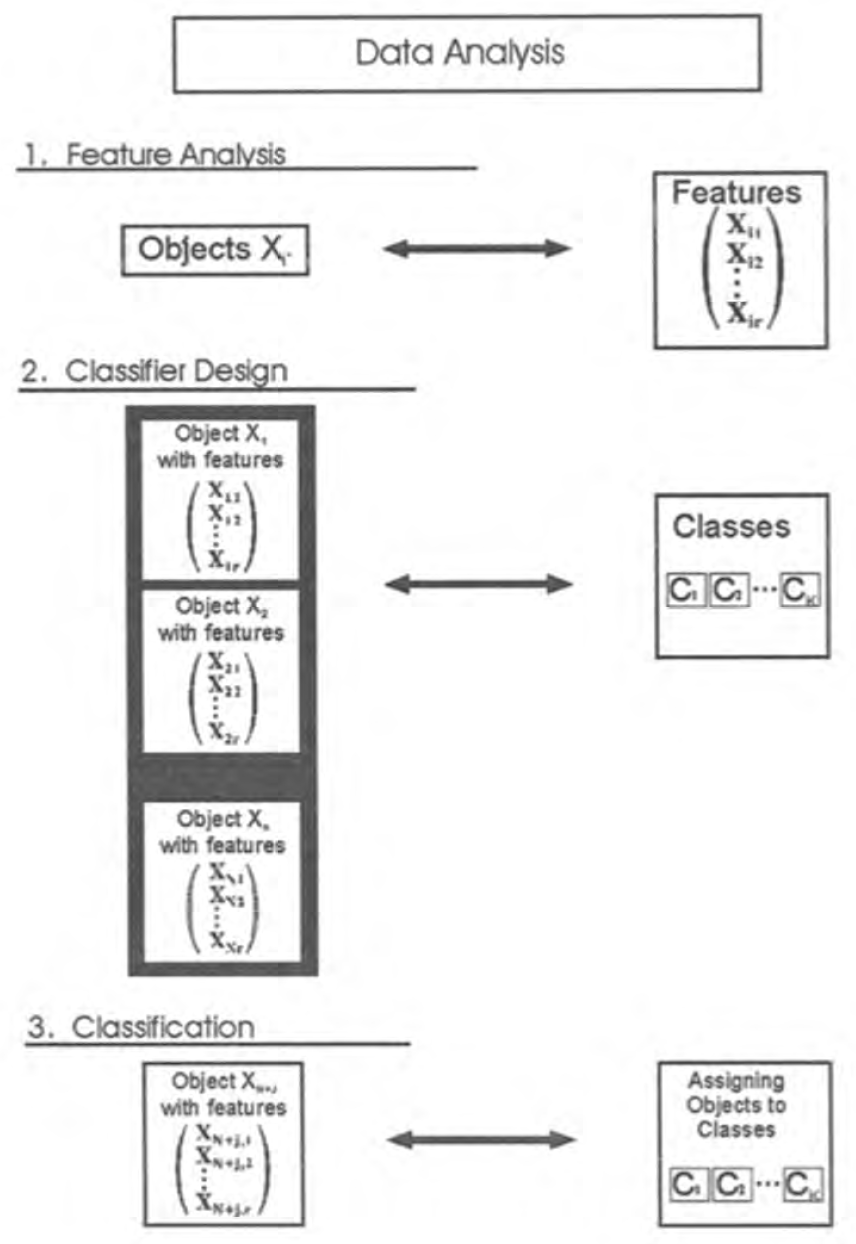
\includegraphics[width=.8\textwidth]{img/sw01/fda.png}
			\end{minipage}
			\hfill
			\begin{minipage}[c]{0.6\textwidth}
				\begin{itemize}
					\item Data analysis can be defined as  \\
						\textbf{search for structure} in data
					\item In data analysis, objects are considered which are described by some attributes
					\item Most of the traditional methods for data analysis assume that patterns to be detected are two-valued
					\item Whenever this is not the case, the relationship between data and classes becomes gradual \\
						$\rightarrow$ Fuzzy Classification
				\end{itemize}
			\end{minipage}
			
			\newpage
			
			\subsubsection{2005 - Data Mining}
			
			\begin{minipage}[c]{0.3\textwidth}
				\centering
				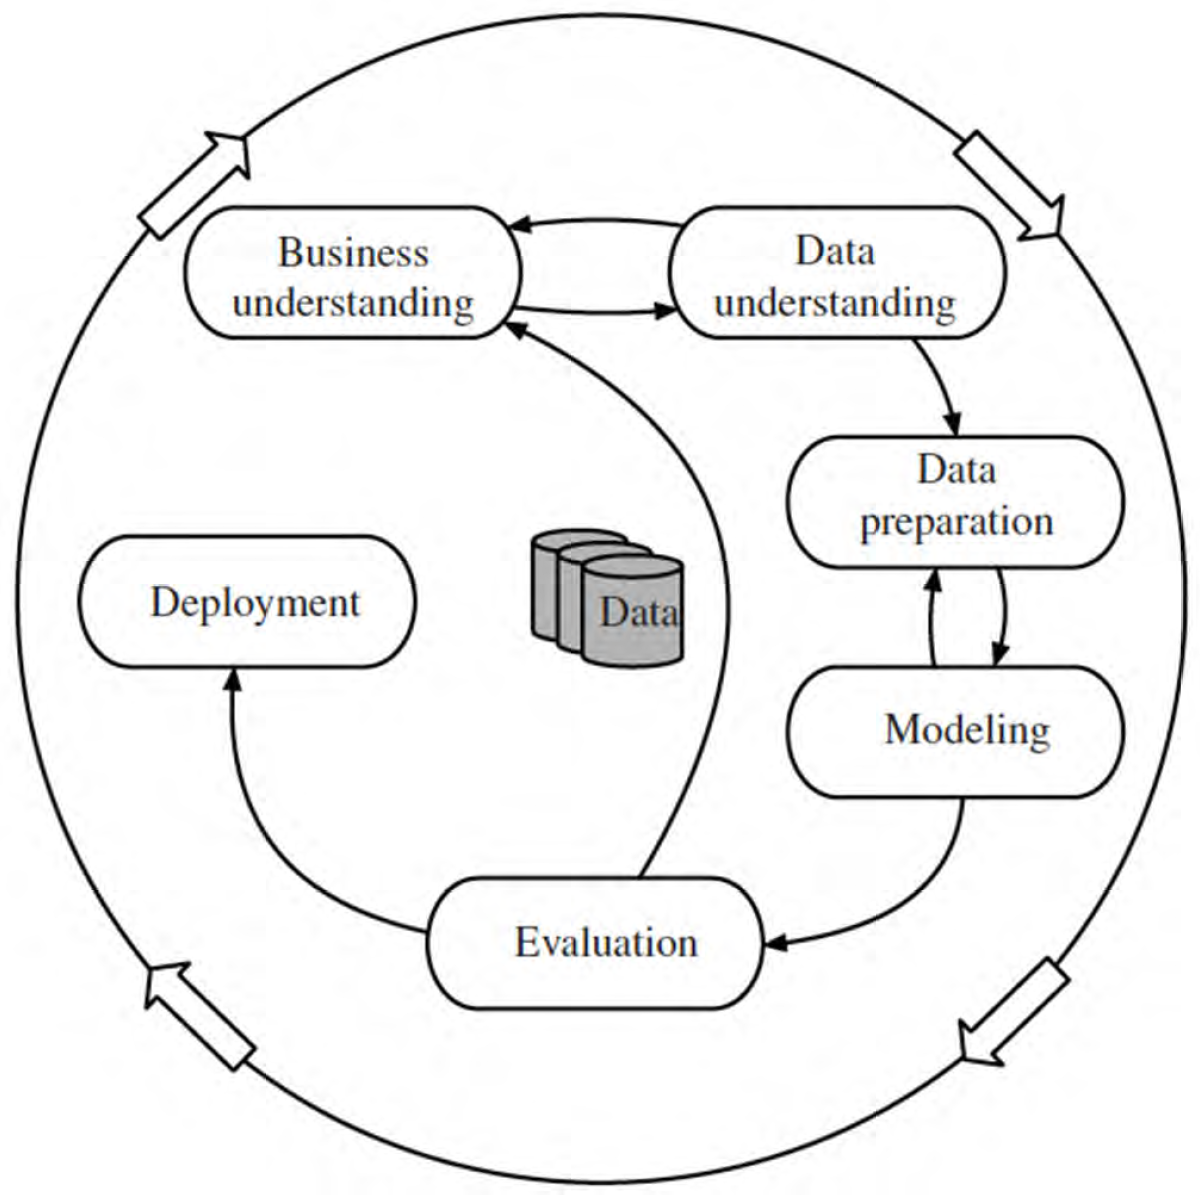
\includegraphics[width=\textwidth]{img/sw01/data-mining.png}
			\end{minipage}
			\hfill
			\begin{minipage}[c]{0.6\textwidth}
				\begin{itemize}
					\item Very similar concept to data science
					\item Machine Learning (modeling) is the technical core of practical data mining applications
					\item Data \textit{Mining} is a business process related to \textit{value} (finding the metaphorical gold nugget)
					\item The lifecycle of a data mining project is defined by the CRISP-DM reference model
				\end{itemize}
			\end{minipage}
		
			\subsubsection{2013 - Predictive Modeling}
			
			\begin{minipage}[c]{0.45\textwidth}
				\centering
				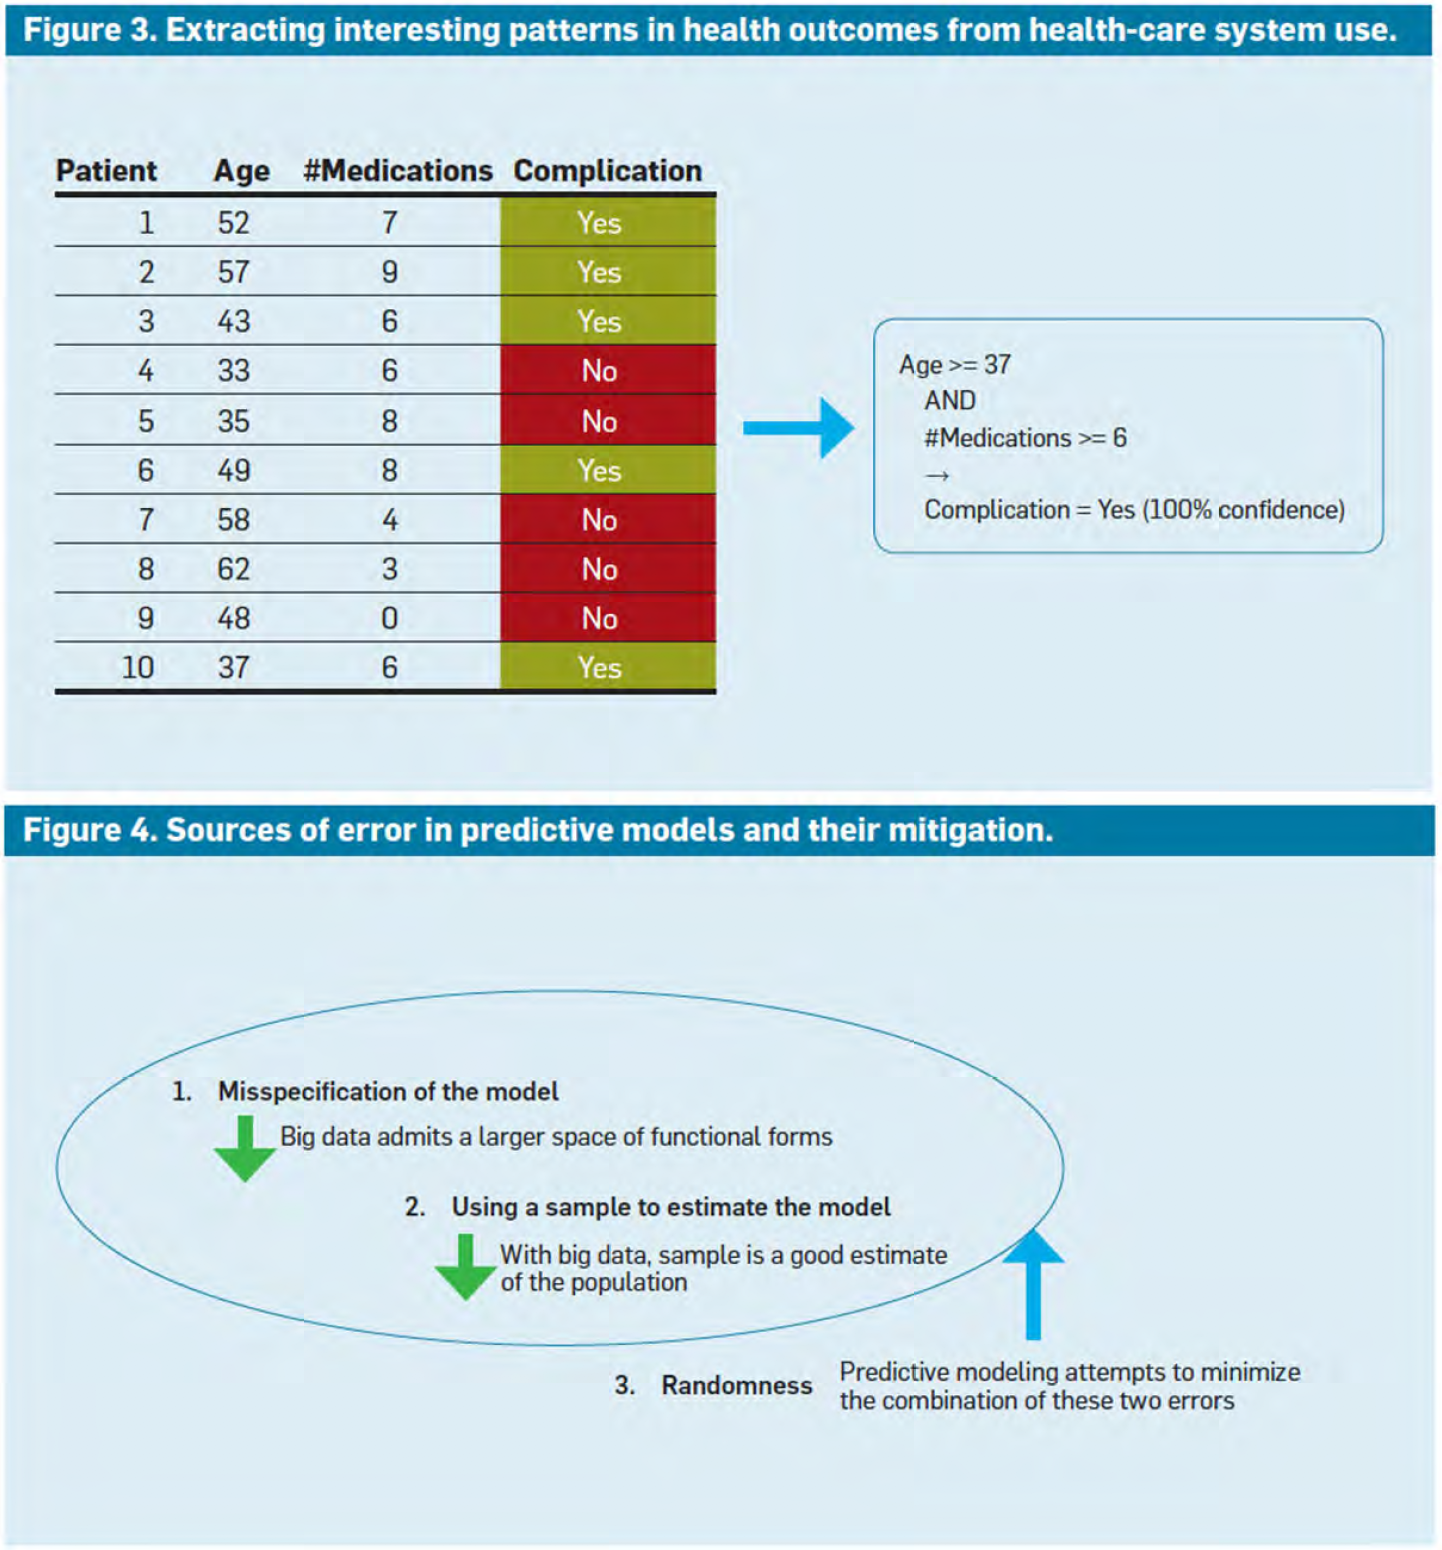
\includegraphics[width=\textwidth]{img/sw01/pred_mod.png}
			\end{minipage}
			\hfill
			\begin{minipage}[c]{0.45\textwidth}
				\begin{itemize}
					\item A common epistemic requirement in assessing whether new knowledge is actionable for decision making in its \textit{predictive power}, not just its ability to explain the past.
					\item The requirement on predictive accuracy on observations that will occur in the future is a key consideration in data science.
				\end{itemize}
			\end{minipage}
		
			\subsubsection{2013 - Data Driven Decision Making}
			
			\begin{minipage}[c]{0.3\textwidth}
				\centering
				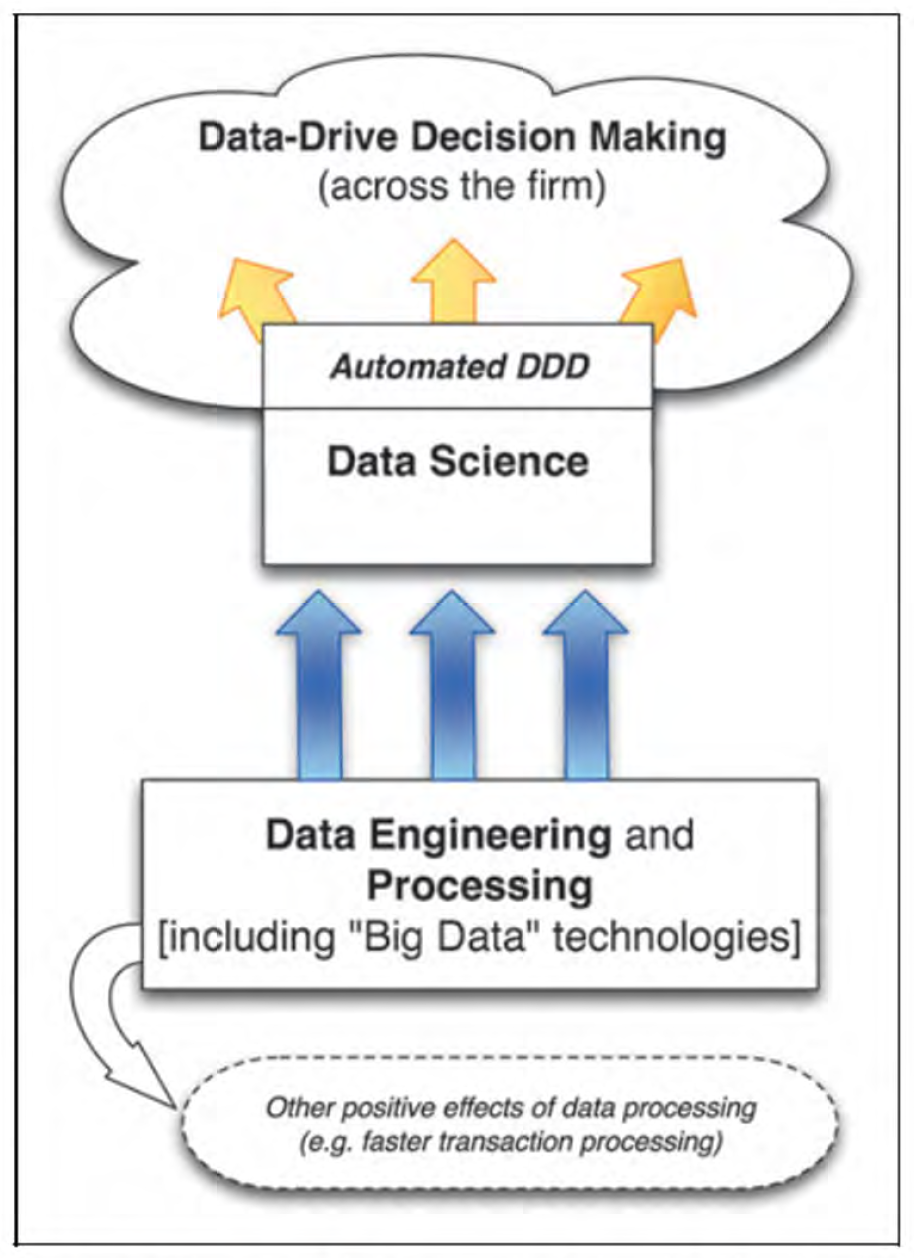
\includegraphics[width=\textwidth]{img/sw01/data_driven.png}
			\end{minipage}
			\hfill
			\begin{minipage}[c]{0.6\textwidth}
				\begin{itemize}
					\item Data science involves much more than just data-mining algorithms.
					\item Successful data scientists must be able to view business problems form a \textit{data perspective}.
				\end{itemize}
			\end{minipage}
		
			\newpage
		
	\section{Intro to R and Exploratory Data Analysis (EDA)}
	
		\subsection{Intro to R}
		
		\begin{itemize}
			\item \textbf{R} ist a software and programming language for statistical applications and graphics
			\item It's an implementation of the programming language S, with some extensions
			\item It provides functions for linear/non-linear modelling, classical statistical tests, time-series analysis, classification, clustering etc.
			\item \textbf{RStudio} is an integrated development environment (IDE) for R
		\end{itemize}
	
			\subsubsection{Basic Operation in R}
			
			\begin{itemize}
				\item Assignment:\\
					\texttt{my\_var <- 46, nr <- 38} \\
					(You can also use \texttt{copy my\_var = 46}, but it is not suggested)
				\item Printing (explicit and implicit): every line with only a name of an object \\
					Implicit: \texttt{my\_var} \\
					Explicit using functions like print: \texttt{print(my\_var)}
				\item Arithmetic operators: \\
					\texttt{4 + 5} \\
					\texttt{2 \^{} 3 - 7 \%\% 3 - 2 \^{} (3 - 7 \%\% 3)} etc. etc. etc.
				\item Control flow, conditionals, loops can be used as in any other language \\
					\texttt{for (i in 1:10) {print(i)}} \\
					\texttt{while (nr < 42) {print("We have "+str(nr)+" : still space..."); nr=nr+1}}
			\end{itemize}
	
		\subsection{What is EDA}
		
		\begin{itemize}
			\item Exploratory Data Analysis is the
				\begin{itemize}
					\item critical process of performing initial investigations on data so as to
						\begin{itemize}
							\item discover patterns
							\item spot anomalies
							\item test hypothesis
							\item check assumptions
						\end{itemize}
					\item with the help of \textbf{summary statistics} and \textbf{graphical representations}
				\end{itemize}
		\end{itemize}
	\noindent
		The use of a statistical model is not mandatory, in this step, even if it is normally adopted to test hypotheses and check assumptions.
		For anomalies and patterns discovery, correlations (represented into the correlation matrix) and distribution (represented with box and whisker diagrams) are the usual approaches.
		
		\begin{figure}[htb!]
			\centering
			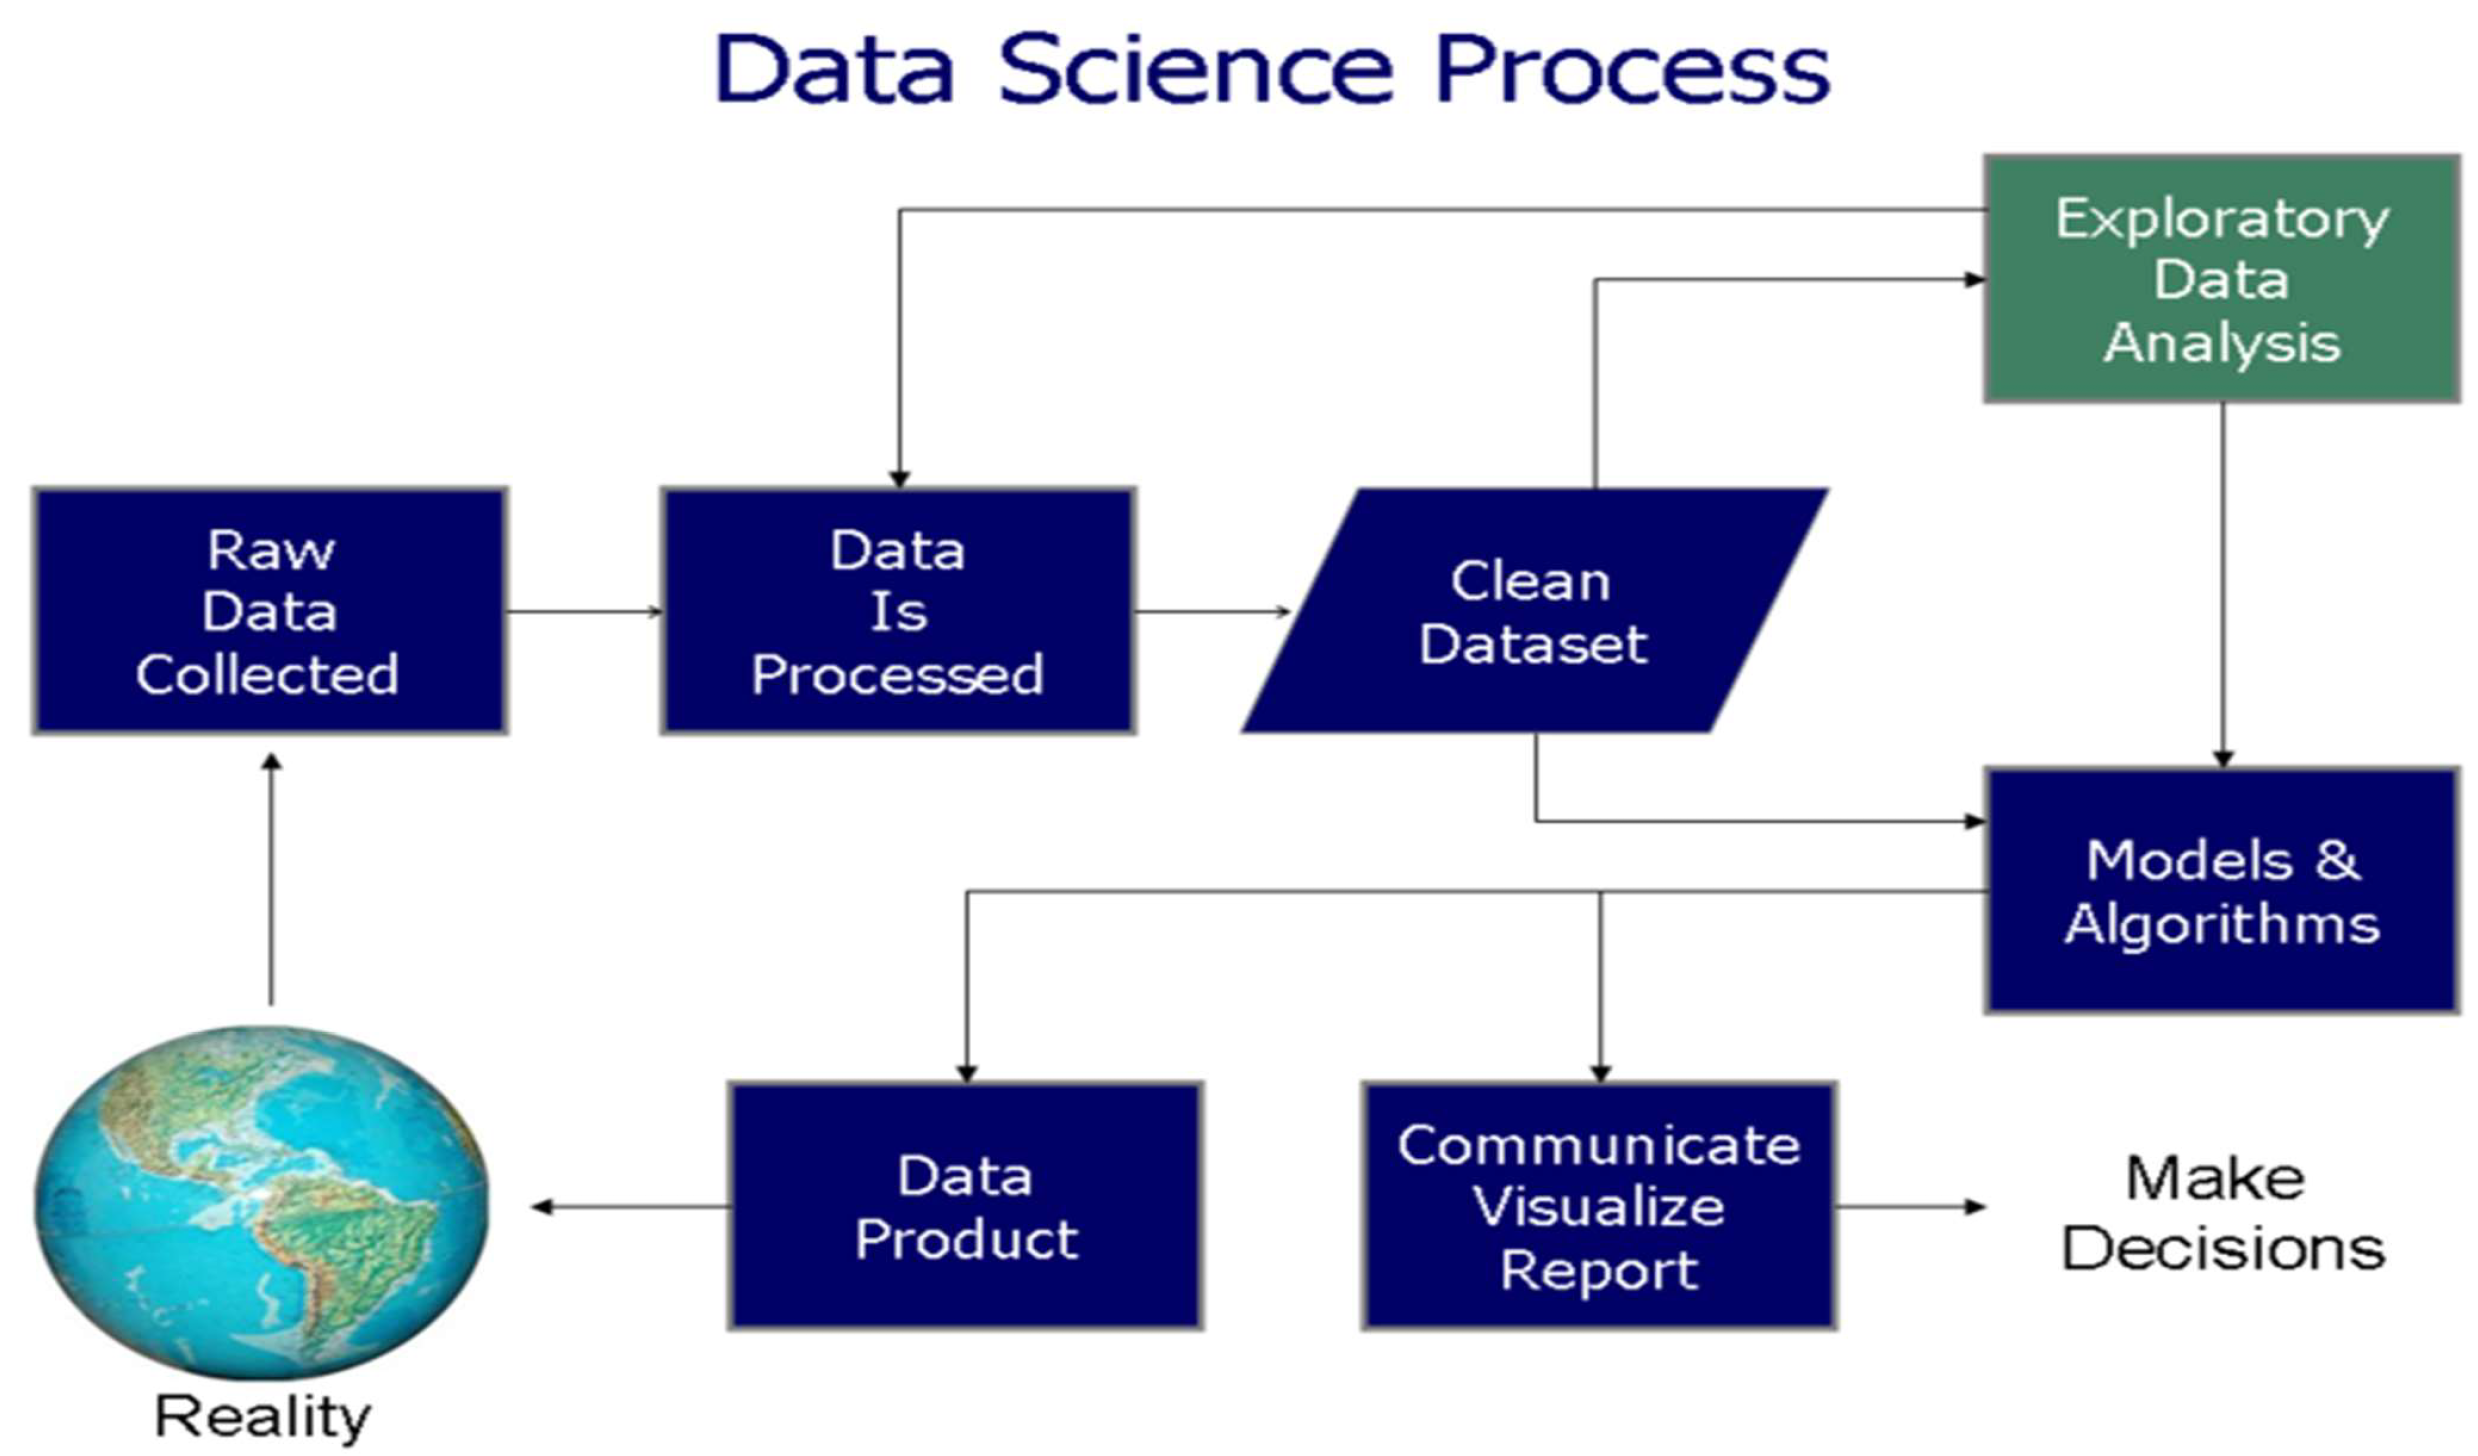
\includegraphics[width=.7\textwidth]{img/sw02/eda_context.png}
			\caption{EDA in the context of Data Science}
		\end{figure}
	
			\newpage
	
			\subsubsection{EDA process "in practice"}
			
			\begin{itemize}
				\item EDA is an iterative cycle
				\item Process:
					\begin{itemize}
						\item Generate questions about the data
						\item Search for answers by visualizing, transforming and modelling the data
						\item Use the insights to refine the questions and/or generate new questions
					\end{itemize}
				\item Start with many ideas...
				\item some will be evidently useless and other will end up in a dead end
				\item a few of them will help to have a better understanding of the data/process
				\item repeat with generating other ideas until the insight is enough
				\item then you can apply the model to the data for forecasting and process explanation
				\item EDA also allows you to verify/test the quality of your data
			\end{itemize}
		
		\subsection{Data Import / Transform / Link}
		
			\subsubsection{Data Import}
			
			\begin{itemize}
				\item R provides importing functions, depending on the format of the data source:
					\begin{itemize}
						\item CSV / TSV / delimited texts: \texttt{read\_csv()} \& \texttt{read\_csv2()} (semicolon), \texttt{read\_tsv()}, \texttt{read\_delim()}
						\item Fixed width columns: \texttt{read\_fwf()} \& \texttt{read\_table()}
						\item Logs (e.g. webserver logs): \texttt{read\_log()}
					\end{itemize}
			\end{itemize}
			These are all similar in terms of parameters, examples:
			
			\begin{lstlisting}
read_delim(file, delim, quote = "\", escape_backslash = FALSE, escape_double = TRUE,
col_names = TRUE, col_types = NULL, locale = default_locale(), na = c("", "NA"),
quoted_na = TRUE, comment = "", trim_ws = FALSE, skip = 0, n_max = Inf, guess_max =
			\end{lstlisting}
			
			\subsubsection{Data Transform (example dataset)}
		
			Example dataset loaded from: \href{https://archive.ics.uci.edu/ml/machine-learning-databases/auto-mpg/}{\textit{\underline{Auto MPG Data Set}}}

			\begin{lstlisting}
> library(tidyverse)
> DS <- read.table("C:/Users/JumpStart/Downloads/auto-mpg.data",
quote="\", comment.char="")
> names(DS) <-
c("mpg","cylinders","displacement","horsepower","weight","acceleration","
model year","origin","car name")
> DS <- as_tibble(DS); attach(DS); View(DS)
			\end{lstlisting}
			
			\newpage
			
			\subsubsection{Data Transform}
		
			\begin{itemize}
				\item Filter rows with \texttt{filter()}
					\begin{itemize}
						\item subset observations based on their values \\
						\texttt{filter(DS, weight > 3500)} or \texttt{filter(DS, DS\$weight > 3500)}
					\end{itemize}
				\item Arrange rows with \texttt{arrange()}
					\begin{itemize}
						\item changes the order of rows \\
						\texttt{arrange(DS, desc(DS\$acceleration))}
					\end{itemize}
				\item Select columns with \texttt{select()}
					\begin{itemize}
						\item Subset columns with position and/or negative condition (by name or index) \\
						\texttt{select(DS, -1)} \\
						\texttt{select(DS, 2, 3, 4)} \\
						\texttt{select(DS, c(mpg, 5))}
					\end{itemize}
				\item Add new variables with \texttt{mutate()} 
					\begin{itemize}
						\item Allow to create new dimension(s) \\
						\texttt{mutate(DS, a4w = acceleration/weight, pre75 = as.numeric(DS\$'model year' < 75))}
					\end{itemize}
				\item Grouped summaries with \texttt{summarise()}
					\begin{itemize}
						\item Allows to compute aggregate metrics \\
						\texttt{summarise(group\_by(DS, 'model year'), mean\_display = mean(displacement), sd\_displ = sd(displacement), n=n()}
					\end{itemize}
			\end{itemize}
			\vspace{1em}
			\begin{itemize}
				\item All verbs work similarly:
					\begin{itemize}
						\item The first argument is a dataframe
						\item The subsequent arguments describe what to do with the data frame, using the variable names (without quotes)
						\item The result is a new data frame
					\end{itemize}
			\end{itemize}
		
			\subsubsection{Data "Linkage"}
			
			Some prices of cars of the 70's: \href{http://www.thepeoplehistory.com/70scars.html}{\textit{\underline{70's Cars}}}. \\
			This data is imported into a new tibble and we will try to use it for creating another View for exploring the relationship between cost, year, power and mpg.
			
			\begin{lstlisting}
> car_cost <-read_delim("C:/Users/JumpStart/switchdrive/__/DASB/SW02/car_197x_costs_2.csv", 
		delim = "-", 
		escape_double = FALSE, 
		na = "NA", 
		trim_ws = TRUE, 
		col_types = cols(`Car Name` = col_factor(), 
		Price = col_character(), 
		Location = col_character(), 
		`Matriculation Year` = col_integer()))
> car_cost <- as_tibble(car_cost)
> car_cost <- mutate(car_cost, Location = sapply(Location,as.factor))
> car_cost <- mutate(car_cost, Price = as.integer(str_replace(str_sub(Price, 2, -1),",","")))
> View(car_cost)
			\end{lstlisting}
	
			\begin{figure}[htb!]
				\centering
				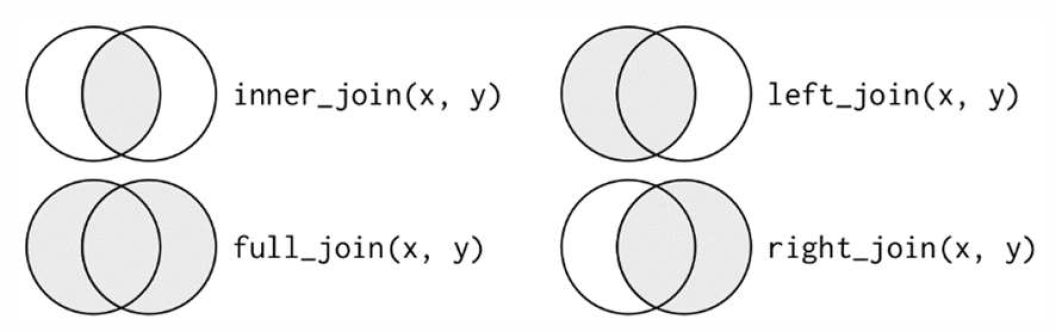
\includegraphics[width=.7\textwidth]{img/sw02/data_linkage.png}
				\caption{R functions to link data frames with each other}
			\end{figure}
	
			\newpage
		\noindent
			There are different types of R functions for linking tibbles/dataframes (\textasciitilde datasets)
					\begin{itemize}
						\item \textbf{Mutating} joins allows to combine variable from two tables
							\begin{itemize}
								\item \texttt{inner\_join(x, y, by = keys)} \\
								matches pairs of observations whenever their keys are equal
								\item Outer join keeps observations that appear in at least one of the tables.
									There are three types of outer joins:
										\begin{itemize}
											\item \texttt{left\_join(x, y, by = keys)} \\
												keeps all observations in x
											\item \texttt{right\_join(x, y, by = keys)} \\
												keeps all observations in y
											\item \texttt{full\_join(x, y, by = keys)} \\
												keeps all observations in x and y
										\end{itemize}
							\end{itemize}
						\item \textbf{Filtering} joins allow to restrict the set of row from the 1$^{st}$ table
							\begin{itemize}
								\item \texttt{semi\_join(x, y, by = keys)} \\
									keeps all observations in x that have a match in y
								\item \texttt{anti\_join(x, y, by = keys)} \\
									drops all observations in x that have a match in y
							\end{itemize}
						\item \textbf{Set Operations} (work on complete rows, comparing each variable values.
							Inputs needs the same variables, for treating observations like sets)
							\begin{itemize}
								\item \texttt{intersect(x, y)} \\
									return only observations in both x and y
								\item \texttt{union(x, y)} \\
									return unique observations in x and y
								\item \texttt{setdiff(x, y)} \\
									return observations in x, but not in y
							\end{itemize}
					\end{itemize}
				
			\subsubsection{Applying data loading/transforming/linking}
			
			\begin{itemize}
				\item Find one or more data sources you are interested into (\href{https://archive.ics.uci.edu/ml/datasets.php}{UCI ML Repository} / \href{https://www.kaggle.com/datasets}{Kaggle})
				\item Start the EDA "mindset":
					\begin{enumerate}
						\item What I believe about the data / what I would like to discover \\
							$\rightarrow$ Make hypotheses and formulate assumptions
						\item Think how this can be supported by data $\rightarrow$ experiment
						\item Run the experiment to verify
						\item Acquire new knowledge that can help you improve step 1
					\end{enumerate}
				\item Repeat the process at least 3 times \\
				\textit{(Optional: short report of the process you followed, document it in a short presentation)}
			\end{itemize}
		
	\section{ggplot2 and its usage in EDA}
	
		\subsection{ggplot2 - Intro}
		
		\begin{itemize}
			\item Used with the library "ggplot2" \\
				\texttt{library(ggplot2)}
			\item Simple usage example: \\
				\texttt{plot <- ggplot(data = mpg, mapping = aes(x = mpg\$hwy))} \\
				plot + geom\_histogram()
			\item ggplot 2 package:
				\begin{itemize}
					\item produces layered statistical graphics.
					\item uses an underlying "grammar" to build graphs layer-by-layer rather than providing premade graphs
					\item is easy enough to use without any exposure to the underlying grammar, but is even easier to use once you know the grammar
					\item allows the user to build a graph from concepts rather than recall of commands and options
				\end{itemize}
		\end{itemize}
	
		\newpage
	
		\subsection{ggplot2 - layer after layer}
		
		\begin{itemize}
			\item The initial call to ggplot does create the graph, but no content: \\
				\texttt{ggplot(data = mpg)} \\
				\texttt{ggplot(data = mpg, mapping = aes(x = mpg\$hwy))} \\
				\texttt{ggplot(data = mpg, mapping = aes(x = mpg\$hwy, y = mpg\$dipl))}
			\item We need to add a layer by using + (or collect the partial graph in an object) \\
				\texttt{p <- ggplot(data = mpg)} \\
				\texttt{p + geom\_histogram(mapping = aes(x = mpg\$hwy))}
			\item Parameters set into the ggplot() call are inherited by every other layer, but can be overridden, if needed \\
				\texttt{p <- ggplot(data = mpg)} \\
				\texttt{p <- p + geom\_histogram(mapping = aees(x = mpg\$hwy))} \\
				\texttt{p} \\
				\texttt{p +  geom\_violin(mapping = aes(y = mpg\$displ))}
		\end{itemize}
	
		\subsection{Elements of grammar of graphics}
		
		\begin{itemize}
			\item \textbf{Data}: variables mapped to aesthetic features of the graph.
			\item \textbf{Geoms}: objects / shapes on the graph.
			\item \textbf{Stats}: statistical transformations that summarize data (e.g. mean, confidence intervals).
			\item \textbf{Scales}: mappings of aesthetic values to data values. 
				Legends and axes visualize scales.
			\item \textbf{Coordinate systems}: the plane on which data is mapped on the graphic.
			\item \textbf{Faceting}: splitting the data into subsets to create multiple variations of the same graph (paneling). 
		\end{itemize}
	
		\subsection{Aesthetics}
		
		\begin{itemize}
			\item Visual properties of objects on the graph (depends on the geom*)
			\item Commonly used aesthetics:
				\begin{description}
					\item[x] positioning along x-axis
					\item[y] positioning along y-axis
					\item[color] color of objects; for 2D-objects: the color of the object's outline (compare to fill below)
					\item[fill] fill color of objects
					\item[linetype] how lines should be drawn (solid, dashed, dotted etc.)
					\item[shape] shape of markers in scatter plots
					\item[size] how large objects appear
					\item[alpha] transparency of objects (value from 0 [transparent] to 1 [opaque])
				\end{description}
		\end{itemize}
	
		\subsection{Geoms}
		
		\begin{itemize}
			\item Geometric shapes produced for the plot.
				\begin{itemize}
					\item \texttt{geom\_bar()}: bars with bases on the x-axis
					\item \texttt{geom\_boxplot()}: boxes and whiskers
					\item \texttt{geom\_density()}: density plots
					\item \texttt{geom\_histogram()}: histogram
					\item \texttt{geom\_line()}: lines
					\item \texttt{geom\_point()}: points (scatterplot)
					\item \texttt{geom\_rug()}: rug plot (2D display with the two 1D marginal distributions)
					\item \texttt{geom\_smooth()}: smoothed conditional means
					\item \texttt{geom\_text()}: text
				\end{itemize}
		\end{itemize}
	
		\newpage
		
		\subsection{Stats \& Scales}
		
		\begin{itemize}
			\item \textbf{Stats} $\rightarrow$ statistically transform data, usually as some form of summary (e.g.: mean, standard deviation, confidence interval etc.).
				Each stat function is associated with a default geom, so no geom is required for shapes to be rendered.
			\item \textbf{Scales} $\rightarrow$ control how a plot maps data values to the visual values of an aesthetic
				\begin{itemize}
					\item \texttt{scale\_color\_manual()}: \\
						define an arbitrary color scale, by scecifying each color manually
					\item \texttt{scale\_color\_hue()}: \\
						define an evenly-spaced color scale, by specifying a range of hues and the number of colors on a scale
					\item \texttt{scale\_shape\_manual()} \\
						define an arbitrary shape scale, by specifying each shape manually
				\end{itemize}
			\item Scales can also be applied to axes:
				\begin{itemize}
					\item \texttt{scale\_x\_continuous()} \\
						map continuous to visual values - \texttt{scale\_x\_discrete()}
					\item \texttt{scale\_x\_date(labels = date\_format("\%m/\%d"), breaks = date\_breaks("2 weeks"))}: \\
						treat x values as dates - scale\_x\_datetime()
					\item \texttt{scale\_x\_log10()}: \\
						plot x on log10 scale
					\item \texttt{scale\_x\_reverse()}: \\
						reverse direction of x-axis
					\item \texttt{scale\_x\_sqrt()}: \\
						plot x on square root scale
				\end{itemize}
		\end{itemize}
	
		\subsection{ggplot2 - Initial Example}
		
		\begin{lstlisting}
ggplot(diamonds, aes(x=carat, y=price, color=cut)) +
	geom_point() +
	scale_color_manual(
	values=c("red", "yellow", "green", "blue", "violet")
) +
scale_y_continuous(
	breaks=c(0,2500,5000,7500,10000,12500,15000,17500),
	labels=c(0,2.5,5,7.5,10,12.5,15,17.5),
	name="price(thousands of dollars)"
)
		\end{lstlisting}
		
		\begin{figure}[htb!]
			\centering
			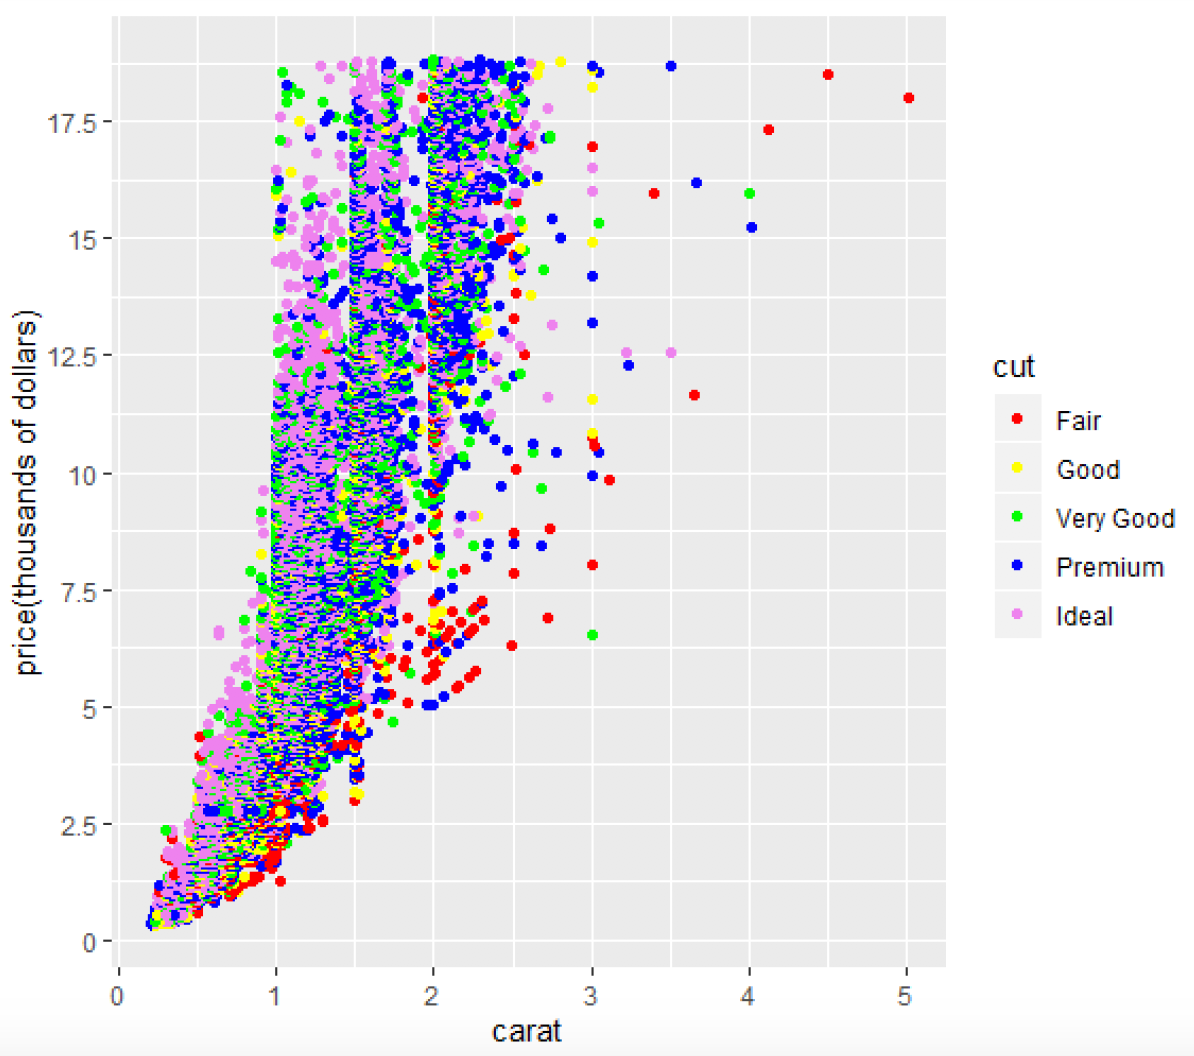
\includegraphics[width=.5\textwidth]{img/sw03/example_01.png}
			\caption{Rendered graph for Initial Example}
		\end{figure}
	
		\newpage
		
		\subsection{Coordinate System \& Faceting}
		
		\begin{itemize}
			\item \textbf{Coordinate system}: set the planes for objects positioning on the plot
			\item Cartesian is the most diffused and used by default.
				Other coordinate systems would be:
				\begin{itemize}
					\item polar
					\item flipped Cartesian
					\item fixed-ratio Cartesian
					\item Map projections (mercatore, lagrange)
				\end{itemize}
			\item \textbf{Faceting}: divide the graph into subgraphs (panels), using variable values
				\begin{itemize}
					\item \texttt{facet\_wrap($\sim$\{vars\})}: \\
						create a multirow panel of plots, \texttt{\{vars\}} represents a list of splitting variables, separated by +
					\item \texttt{facet\_grid(\{vars\}$\sim$\{vars\})}: \\
					row-splitting variable before, the column-splitting variable after
				\end{itemize}
			\item Other aspects include the teming, position adjustment, labels and legends, zooming and the graph savings (ggsave)
		\end{itemize}
	
		\subsection{ggplot2 - Second Example}
		
		\begin{lstlisting}
ggplot(diamonds, aes(x=carat, y=price, color=cut)) +
	geom_point() +
	facet_grid(clarity~color) +
	scale_color_manual(values=c("red", "yellow", "green", "blue", "violet")) +
	scale_y_continuous(breaks=c(0,2500,5000,7500,10000,12500,15000,17500),
	labels=c(0,2.5,5,7.5,10,12.5,15,17.5),name="price(thousands of dollars)")
		\end{lstlisting}
		
		\begin{figure}[htb!]
			\centering
			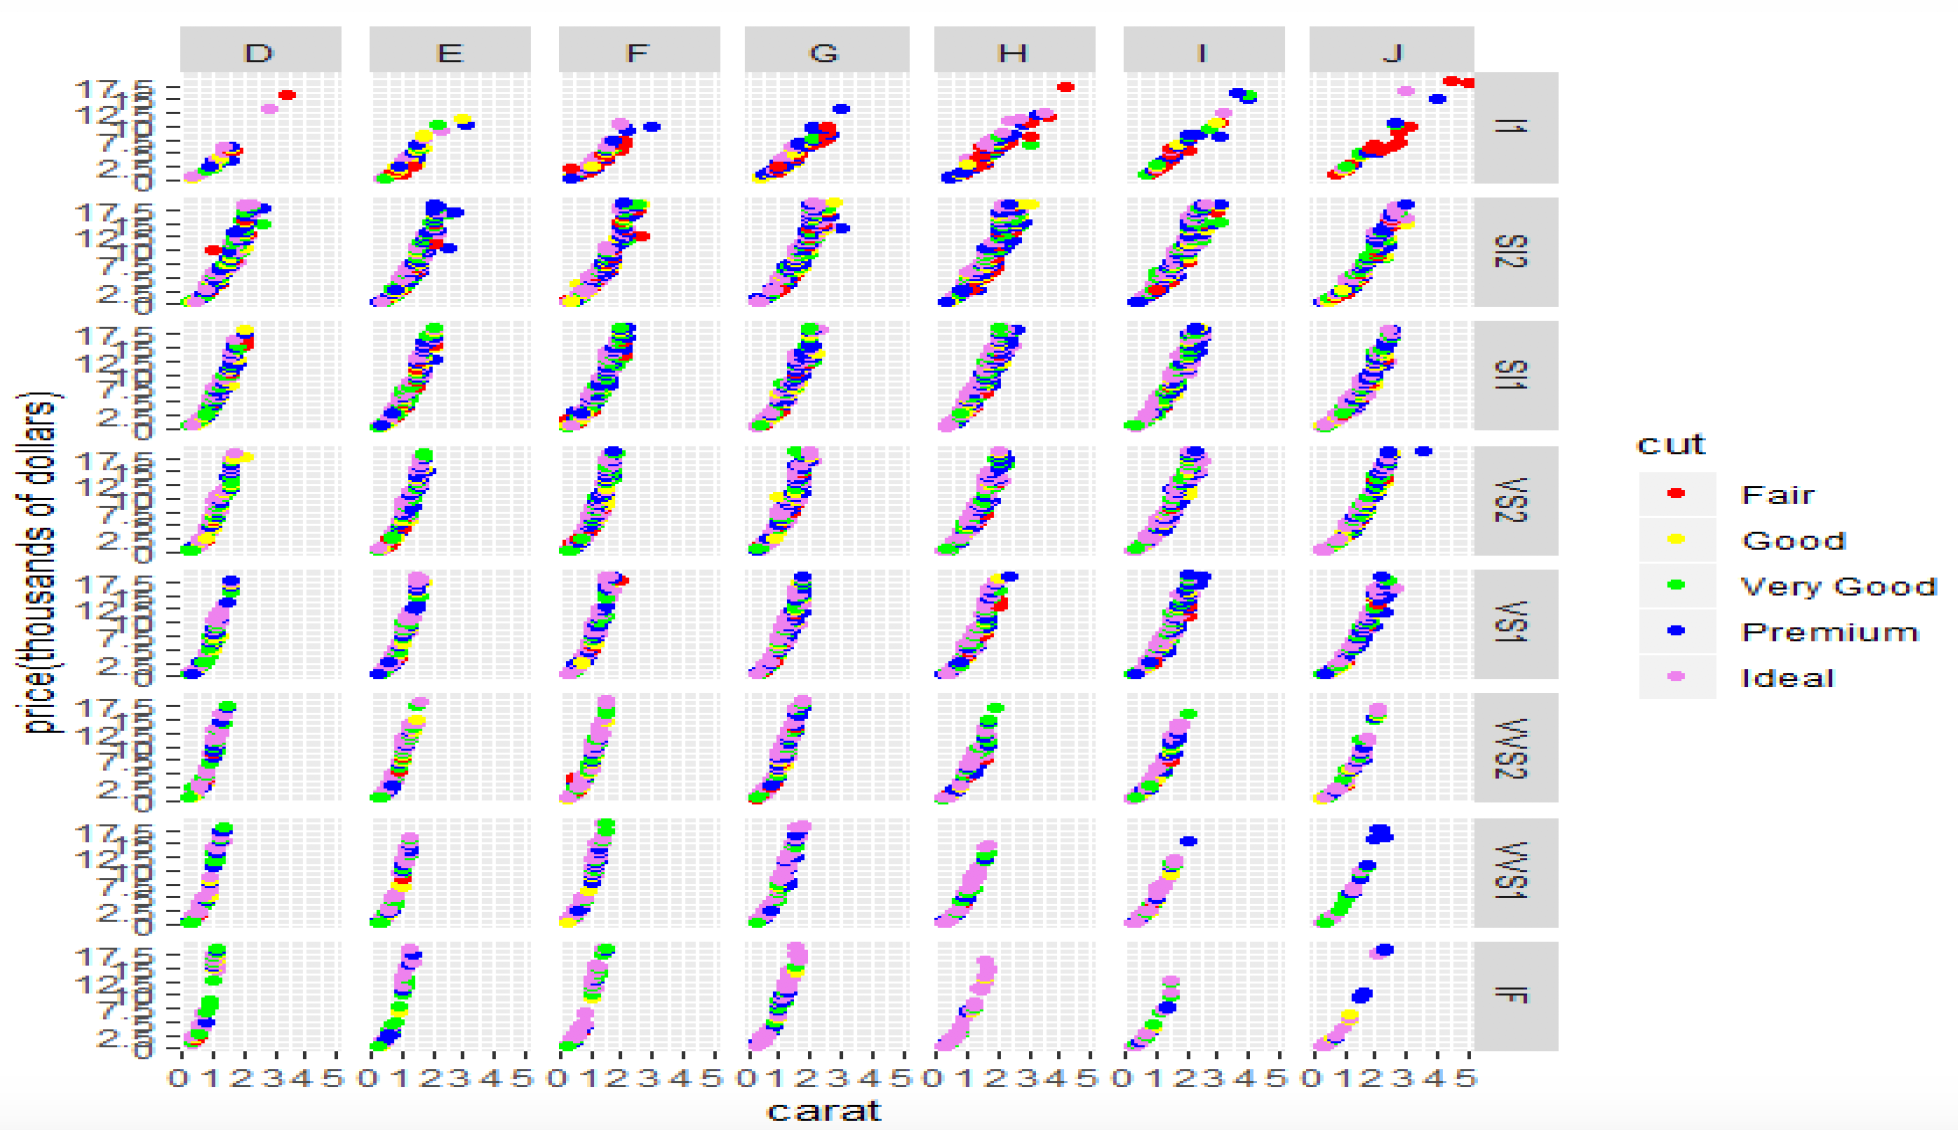
\includegraphics[width=.8\textwidth]{img/sw03/example_02.png}
			\caption{Rendered graph for Second Example}
		\end{figure}
	
		\newpage
		
	\section{Shiny}
	
	Machi de wenni no Loscht han.
	(Wenn de Text am Schloss no do esch, hani kei Loscht meh gha)
	%TODO
	
	\section{Intro to Forecasting}
	
		\subsection{Indication}
		
		\begin{itemize}
			\item Forecast: the ability to use a set of variables for predicting another one
			\item Predictors $\rightarrow$ $F(x)$ $\rightarrow$ Output
			\item Can assume two forms:
				\begin{itemize}
					\item Continuous Output $\rightarrow$ Regression
					\item Discrete (Categorical) Output $\rightarrow$ Classification
				\end{itemize}
			\item It uses similar approaches, but with a different result
			\item The function $F(x)$ is called the model.
				Can be used for two goals:
				\begin{itemize}
					\item Pure prediction: care only for the forecast
					\item Interpretation: care of the existing relationship, to better understand the phenomena
				\end{itemize}
		\end{itemize}
	
		\subsection{Linear Modeling}
		
			\subsubsection{Modeling}
			
			\begin{itemize}
				\item Simplest form of a model is the Linear Model
				\item With one predictor (bidimensional space) represent the equation of a line: \\
					$ y = F(x) = \beta_0 + \beta_1 \cdot x $ \\
			\end{itemize}
		
			\begin{minipage}[c]{0.4\textwidth}
				\centering
				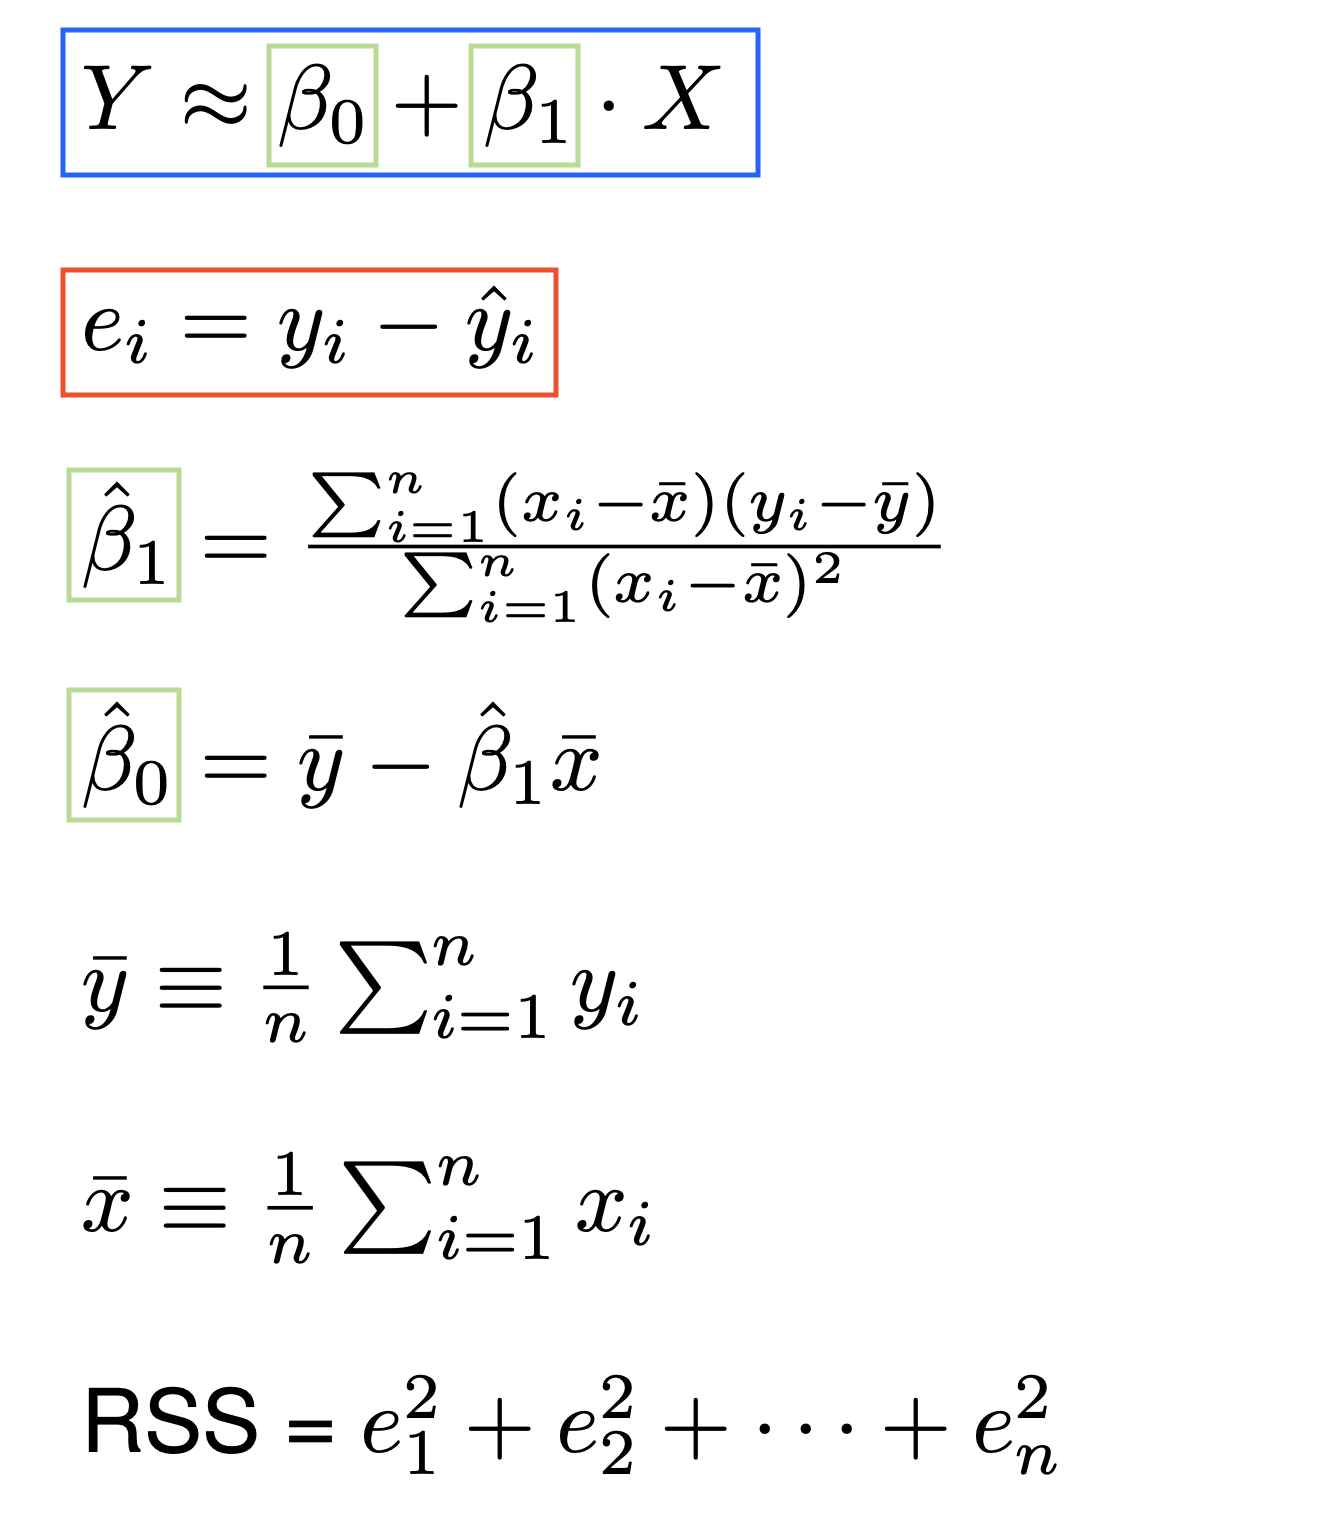
\includegraphics[width=\textwidth]{img/sw08/linear_equations.png}
			\end{minipage}
			\hfill
			\begin{minipage}[c]{0.5\textwidth}
				\centering
				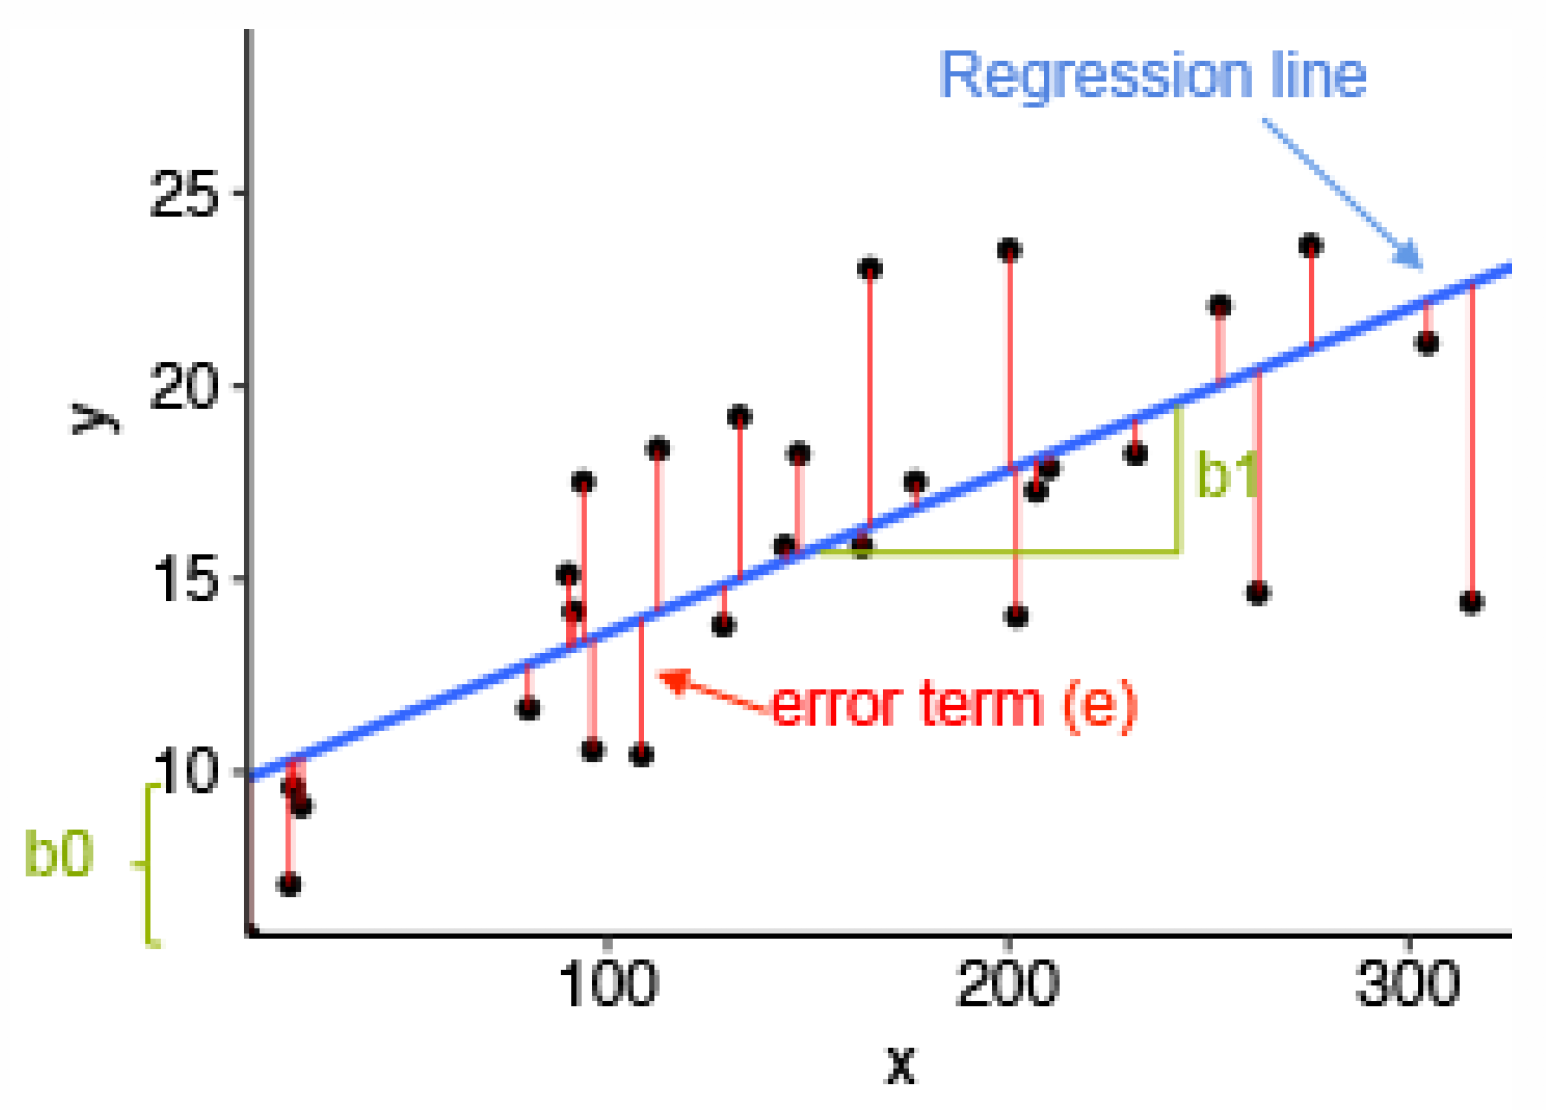
\includegraphics[width=\textwidth]{img/sw08/linear_model.png}
			\end{minipage}
		
			\begin{itemize}
				\item With more predictors (multidimensional space or Hyperspace), \\
					the model can be seen as a hyperplane: \\
					$ y = F(x) = \beta_0 + \beta_1\cdot + \beta_2 \cdot x_2 + \dots + \beta_n \cdot x_n $
			\end{itemize}
		
			\begin{figure}[htb!]
				\centering
				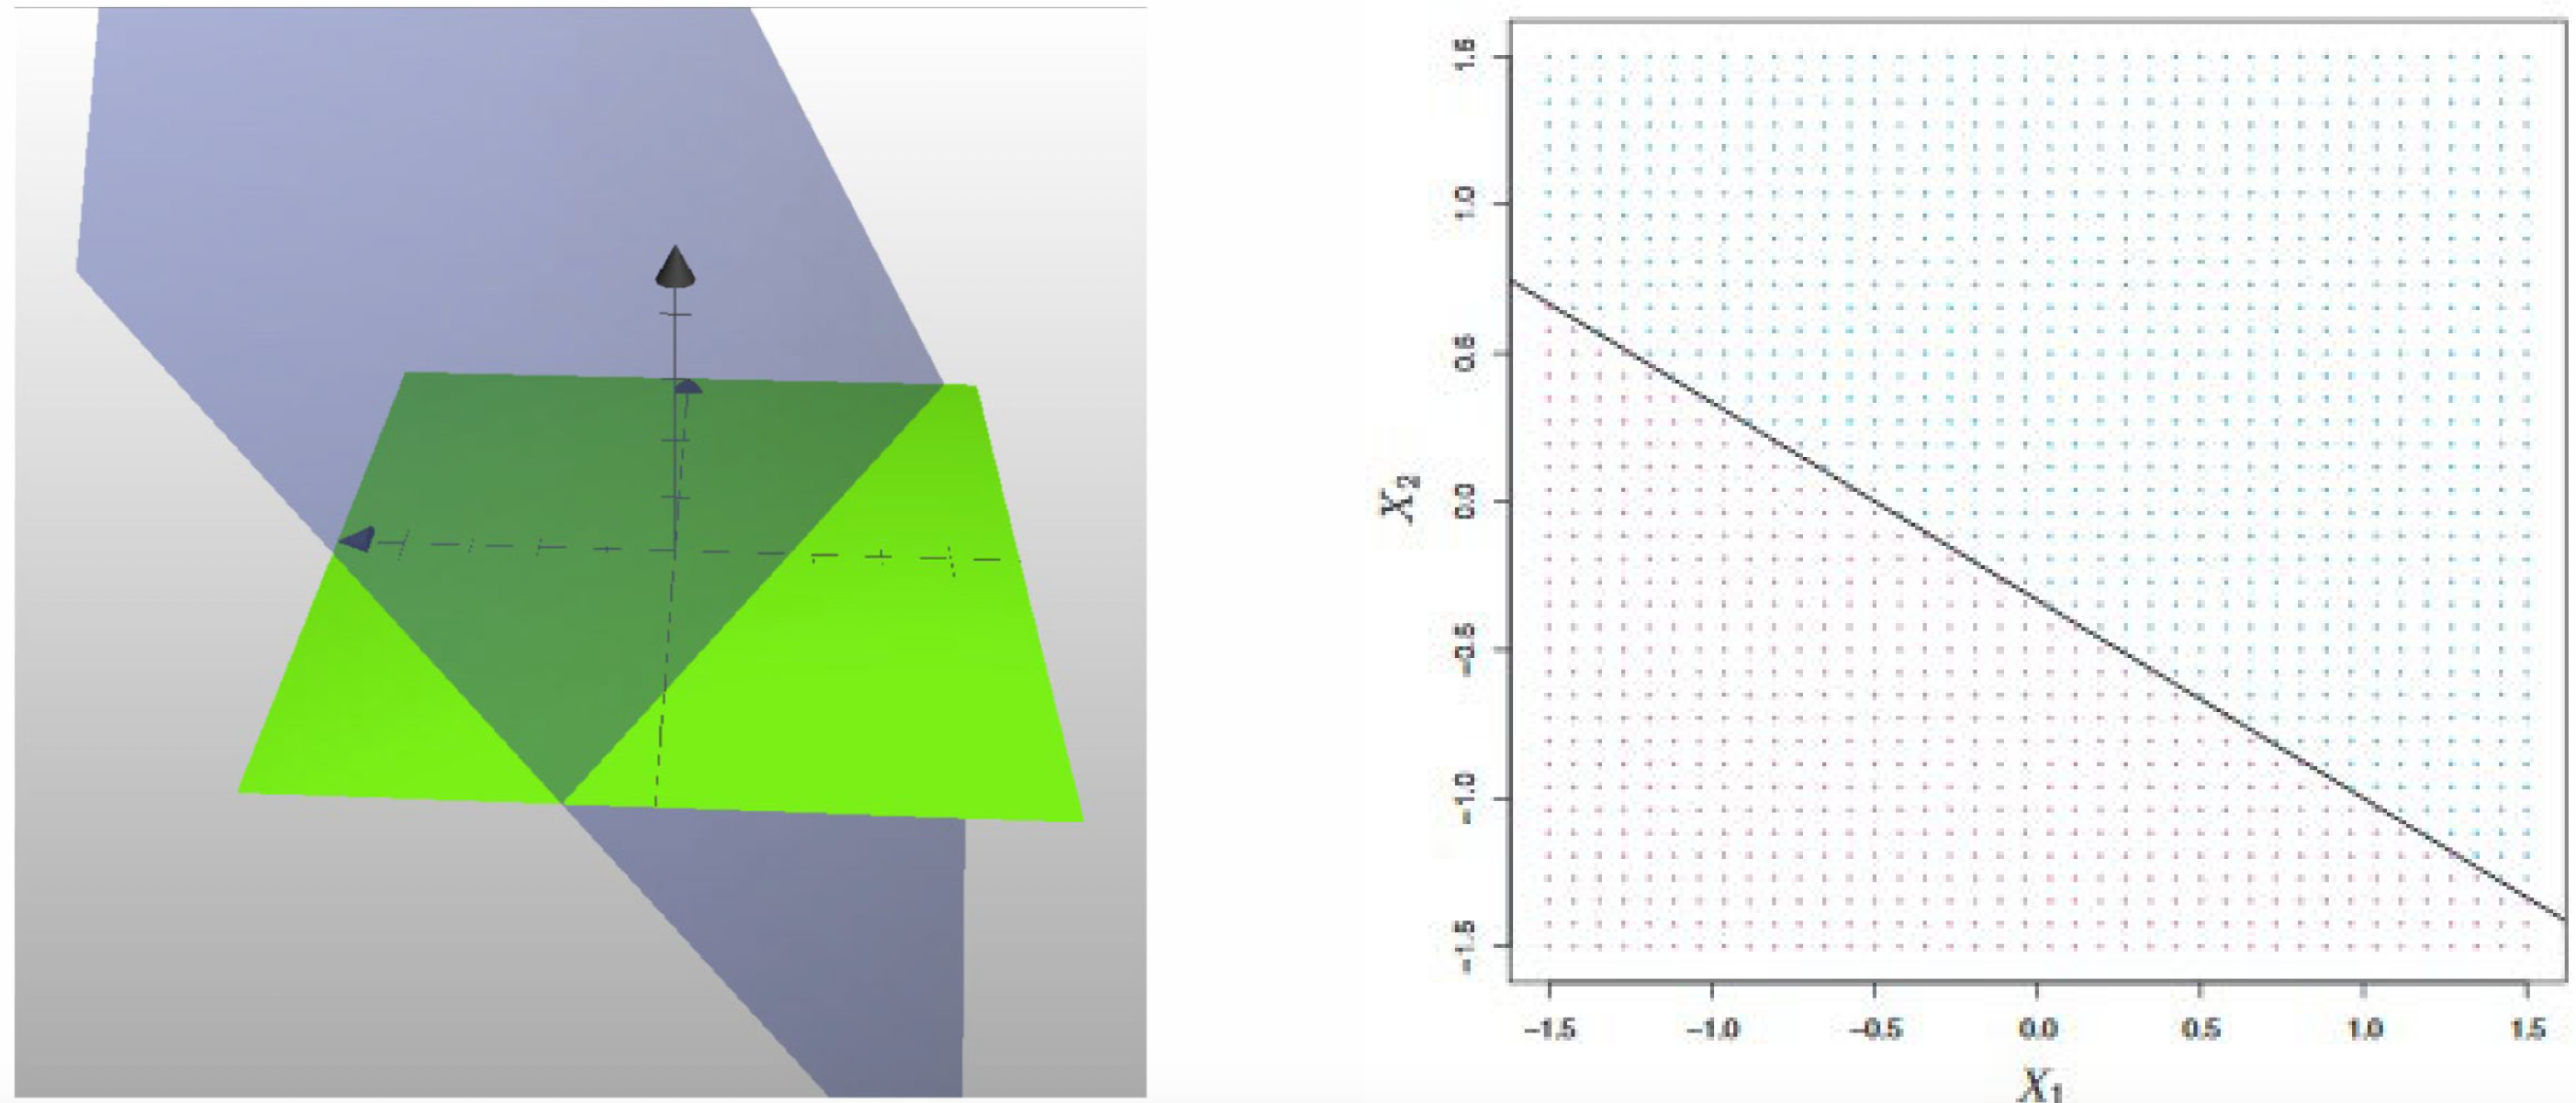
\includegraphics[width=.65\textwidth]{img/sw08/hyperplane.png}
			\end{figure}
		
			\newpage
			
			\subsubsection{Model Identification}
			
			Following steps need to be done
				\begin{itemize}
					\item Define the predictors set and the output variables (also using correlation)
						\begin{itemize}
							\item $x = \dots$, $y = \dots$
						\end{itemize}
					\item Create the model
						\begin{itemize}
							\item \texttt{model <- lm(y \textasciitilde{} x, data = d)}
						\end{itemize}
					\item Inspect the model
						\begin{itemize}
							\item Parameters $\beta_0, \beta_1, \beta_2, \dots, \beta_n$
						\end{itemize}
					\item Verify that the model is "trustable"
						\begin{itemize}
							\item P-values of each $\beta_a$, everyone should be under 0.05 (5\%)
						\end{itemize}
				\end{itemize}
			
			\subsubsection{Prediction}
			
			\begin{itemize}
				\item It is natural to interpret the model for regression:
					\begin{itemize}
						\item Given a single set of predictor values $X$ (point) $\rightarrow$ compute the value of the output ($y$)
					\end{itemize}
				\item but what about for classification?
					\begin{itemize}
						\item We need to define a way to transform the output of the linear model to our output categories
						\item This is done by the logistic function
					\end{itemize}
				\item How to do predictions:
					\begin{itemize}
						\item \texttt{Pred <- predict(model, data = d2)}
					\end{itemize}
			\end{itemize}
				
			\begin{figure}[htb!]
				\centering
				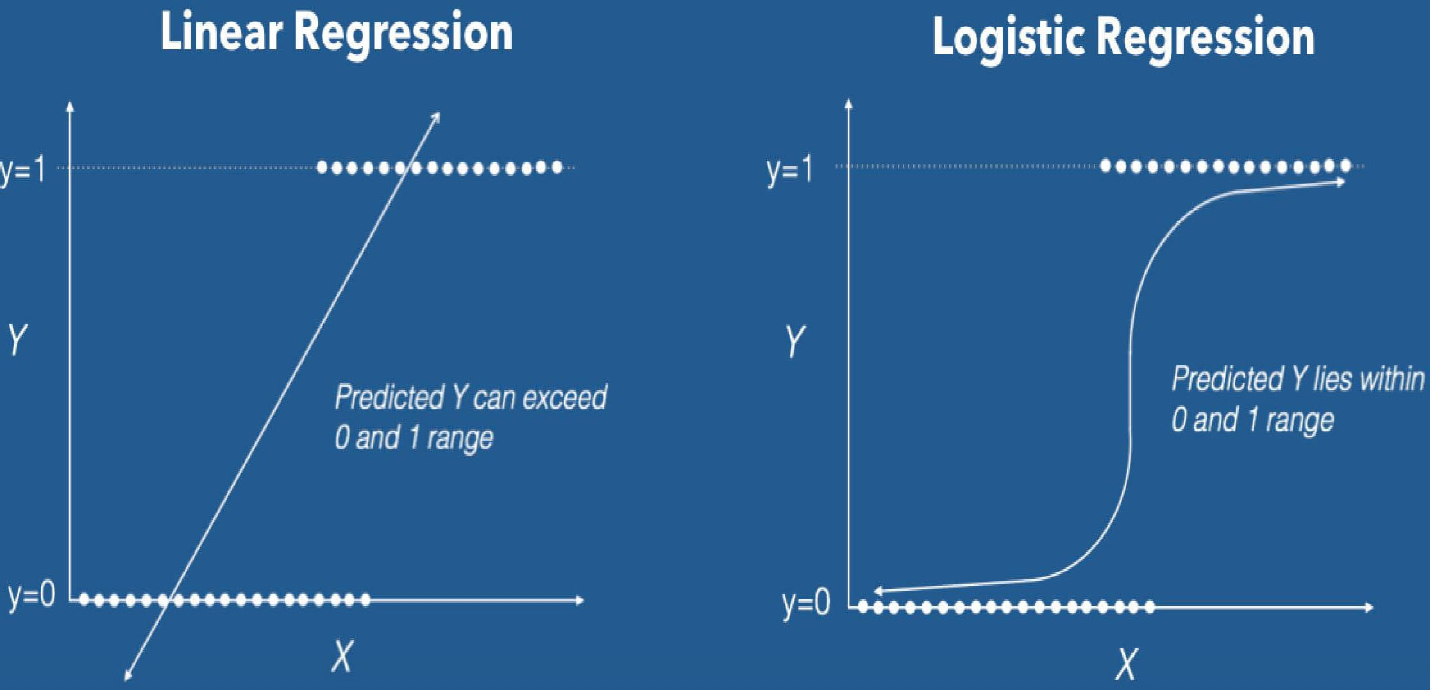
\includegraphics[width=.6\textwidth]{img/sw08/prediction.png}
			\end{figure}
		
			\subsubsection{Model Evaluation}
			
			\begin{itemize}
				\item We need to evaluate models based on performances
					\begin{itemize}
						\item Regression $\rightarrow$ the sum of squared errors (RSS $\rightarrow$ residual sum of squares)
						\item Classification $\rightarrow$ the misclassification error rate
					\end{itemize}
				\item Every model with more predictors has a higher predictive power... \\
					...but, we don't want to learn the noise on the data!
				\item Create an independent test set
					\begin{itemize}
						\item Use most part (e.g. 70\%) of the data for training purposes
						\item Use the rest for the model performance estimation $\rightarrow$ Test Error Rate
					\end{itemize}
			\end{itemize}
		
			\newpage
				
	\section{Forecasting Models: Usage / Application}
	
		\subsection{Forecasting vs. Interpretation}
		
		\begin{itemize}
			\item Linear model
				\begin{itemize}
					\item Rigid (strong assumptions about the relationship)
						\begin{itemize}
							\item Predictors can only be represented by variables
							\item Predictors do not have interactions (can be analyzed separately)
						\end{itemize}
					\item $y = F(X) = \beta_0 + \beta_1 x_1 + \dots + \beta_n x_n$
				\end{itemize}
			
			\item Two extensions:
				\begin{itemize}
					\item  Transformation applied to variables, to be used as predictor and/or output
						\begin{itemize}
							\item E.g.: $\log_2(y) = F(X) = \beta_0+ \beta_1 \sin x_1 + \dots + \beta_n e^{x_n}$
							\item Formula $\rightarrow$ $y \sim I(\sin(x_1)) + \dots + I(\exp(x_n))$
						\end{itemize}
					\item Interaction between variables
						\begin{itemize}
							\item E.g.: $y = F(X) = \beta_0 + \beta_1 x_1 + \beta_2 x_2 + \beta_{1\_2} x_1 x_2$
							\item Formula $\rightarrow$ $y \sim x_1 \cdot x_2$
						\end{itemize}
				\end{itemize}
		\end{itemize}
	
		\subsection{Performance vs. Interpretability}
		
		\begin{itemize}
			\item Every extension adds more predictive performances, but reduces interpretability.
			\item Limits (boxes between Input $\rightarrow$ $\dots$ $\rightarrow$ Output):
				\begin{itemize}
					\item Pure linear model $\rightarrow$ white box
					\item Complex extensions $\rightarrow$ black box
					\item Intermediate $\rightarrow$ gray boxes
				\end{itemize}
		\end{itemize}
	
		\subsection{Parametric vs. non-Parametric models}
		
		\begin{itemize}
			\item All linear models (ad extensions) are called \textbf{parametric} models:
				\begin{itemize}
					\item They make assumptions on the data distribution
					\item Are bound to the amount they can learn, depending on the fixed number of parameters of the model
					\item Other examples of parametric models are: \\
					Logistic Regression, Polynomial Regression and Perception
					\item A learning model that summarizes data with a et of parameters of fixed size (independent of the number of training examples) is called a parametric model.
					No matter how much data you throw at a parametric model, it won't change its mind about how many parameters it needs.
				\end{itemize}
			\item More complex models from Machine Learning are \textbf{non-parametric}:
				\begin{itemize}
					\item Nonparametric methods are good when you have a lot of data and no prior knowledge, 
						and when you don't want to worry too much about choosing just the right features.
					\item The amount of information that the model is able to capture can grow with the increase in the amount of data analysed.
					\item Examples of non-parametric models are: k-Nearest Neighbors (kNN), Decision Trees, Support Vector Machines, Neural Networks
					\item They are normally more powerful (predictive power), but their interpretation is limited or basically impossible.
				\end{itemize}
		\end{itemize}
			
			\newpage
				
			\subsubsection{Pros and Cons (Param vs. non-Param)}
			
			\begin{figure}[htb!]
				\centering
				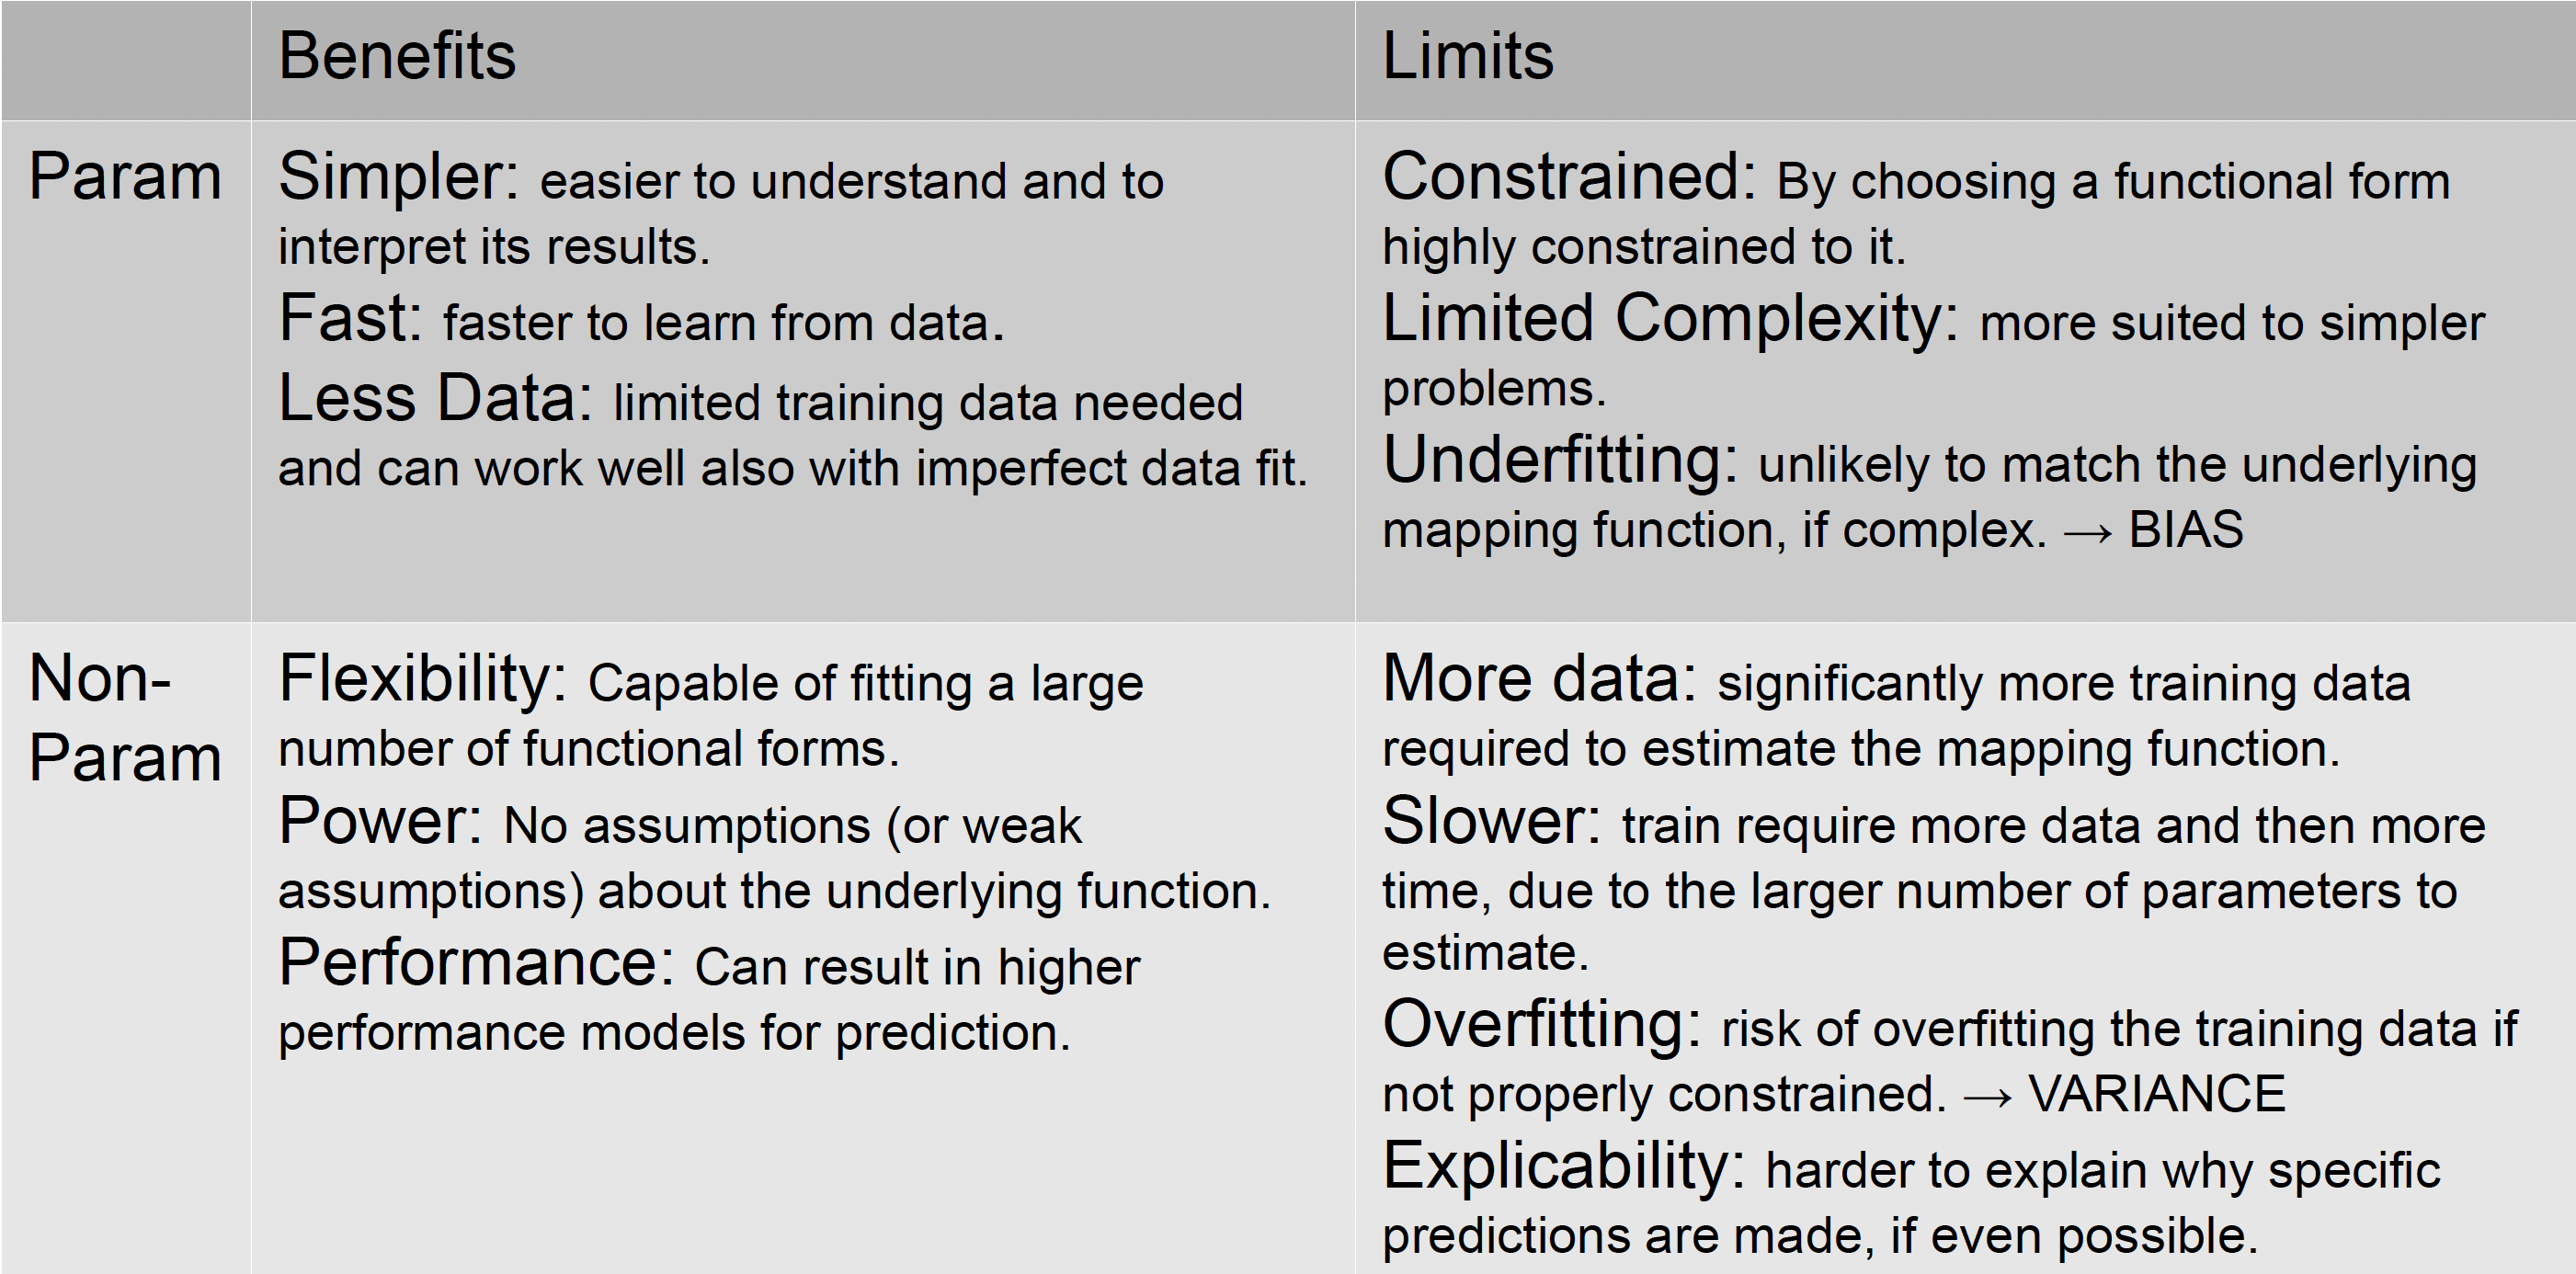
\includegraphics[width=\textwidth]{img/sw09/pro_con.png}
			\end{figure}
		
			Rigidness (Bias) vs. Instability/Sensibility to data (Variance) tradeoff.
			It depends on:
			\begin{itemize}
				\item the amount of data
				\item the complexity and the underlying function/relationship to estimate
			\end{itemize}
		
		\subsection{General approach to ML / Data Science}
		
		Mathwork guides about ML: \href{https://ch.mathworks.com/content/dam/mathworks/tag-team/Objects/i/88655_93014v00_machine_learning_section2_ebook.pdf}{Guide 1} and
		\href{https://ch.mathworks.com/content/dam/mathworks/tag-team/Objects/i/90221_80827v00_machine_learning_section4_ebook_v03.pdf}{Guide 2}
		
		\begin{figure}[htb!]
			\centering
			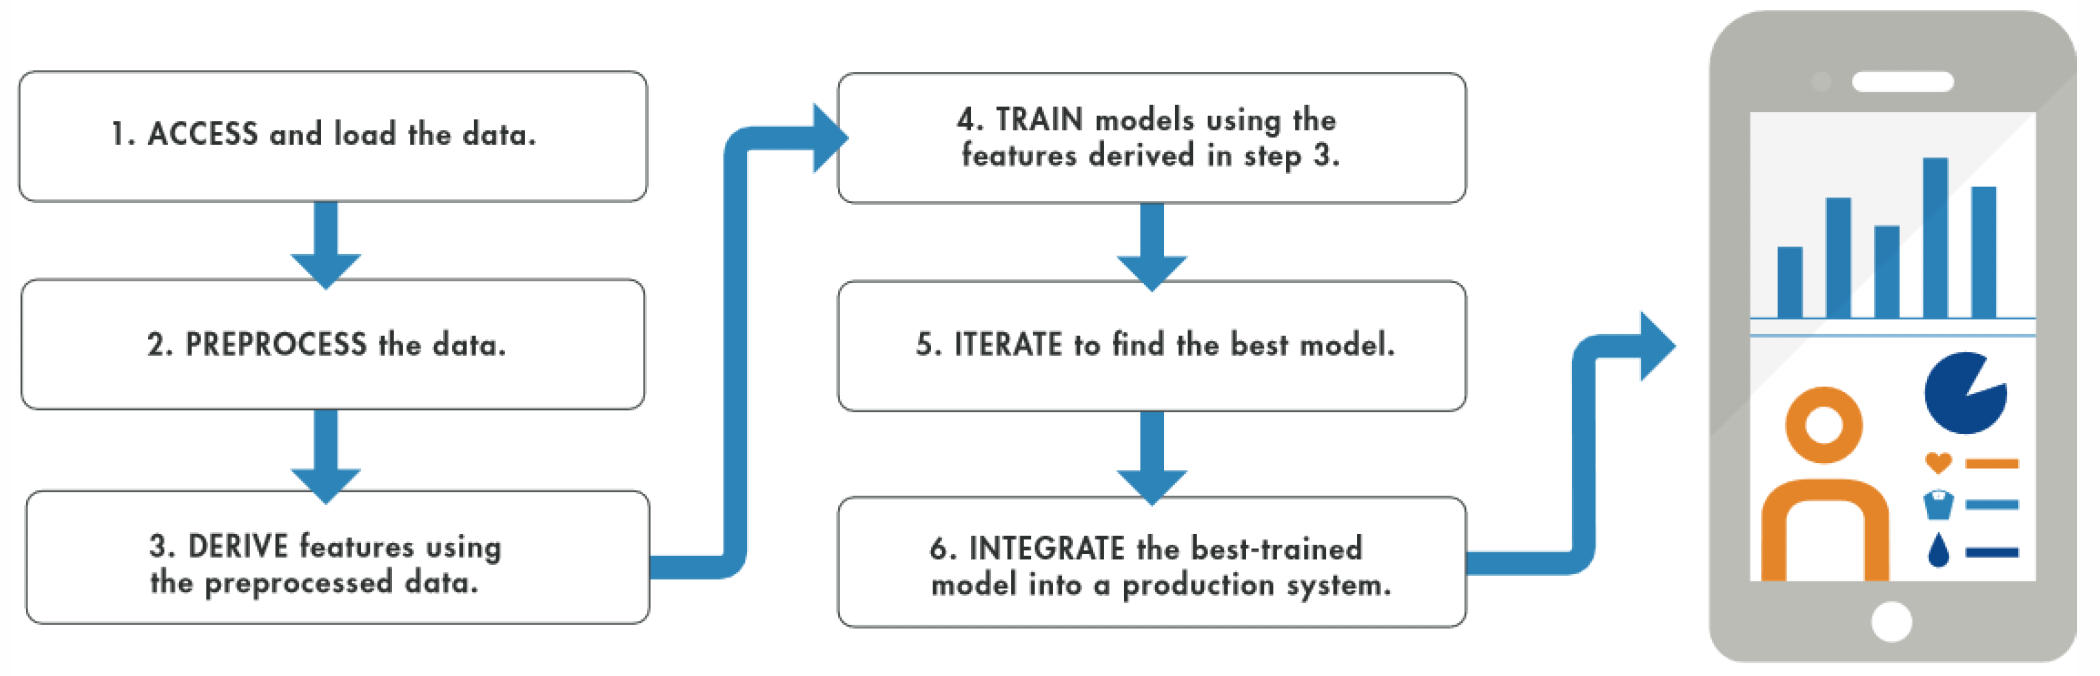
\includegraphics[width=\textwidth]{img/sw09/ml_approach.png}
		\end{figure}
	
		\subsection{An example (yup, that's the title)}
		
		\begin{itemize}
			\item This example is based on a cell phone health-monitoring app.
			\item The input consists of three-axial sensor data from the phone's accelerometer and gyroscope.
			\item The responses (or output) are the activies performed: walking, standing, running, climbing stairs or lying down.
				\begin{itemize}
					\item \textbf{Supervised} = we have the classes
					\item  \textbf{Unsupervised} = we would like to discover some structure, but don't have a real output variable
				\end{itemize}
			\item Supervised $\rightarrow$ Classification
				\begin{itemize}
					\item The trained model (or classifier) will be integrated into an app to help users track their activity levels throughout the day.
				\end{itemize}
		\end{itemize}
	
		\newpage
		
		The five steps:
		\begin{itemize}
			\item Step 1: Load the data
			\item Step 2: Preprocess the data
			\item Step 3: Derive features (predictors)
			\item Step 4: Build and train the model
			\item Step 5: Improve the model
		\end{itemize}
	
			\subsubsection{Step 1: Load the Data}
			
			\begin{itemize}
				\item To load data from the accelerometer and gyroscope, we need to do the following:
					\begin{enumerate}
						\item Sit down holding the phone, log data from the phone, and store it in a text file labeled "Sitting".
						\item Stand up holding the phone, log data from the phone, and store it in a second text file labeled "Standing".
						\item Repeat the steps until we have data for each activity we want to classify.
					\end{enumerate}
				\item We store the labeled data sets in a text file.
				\item A flat file format such as text or CSV is easy to work with and makes it straightforward to import data.
				\item Machine learning algorithms are not smart enough to tell the difference between noise and valuable information.
				\item Before using the data for training, we need to make sure it's clean and complete.
			\end{itemize}
		
			\subsubsection{Step 2: Preprocess the data}
			
			\begin{itemize}
				\item We import the data into our environment and plot each labeled set.	
					To preprocess the data we do the following:
					\begin{enumerate}
						\item Look for outliers $\rightarrow$ data points that lie outside the rest of the data
							\begin{itemize}
								\item We must decide whether the outliers can be ignored or whether they indicate a phenomenon that the model should account for.
								\item In our example, they can safely be ignored (it turns out that we moved unintentionally while recording the data).
							\end{itemize}
						\item Check for missing values (perhaps we lost data because the connection dropped during recording).
							\begin{itemize}
								\item We could simply ignore the missing values, but this will reduce the size of the data set.
									Alternatively, we could substitute approximations for the missing values by interpolating or using comparable data from another sample (data augmentation).
							\end{itemize}
						\item Remove gravitational effects from the accelerometer data so that our algorithm will focus on the movement of the subject, not the movement of the phone.
							A simple high-pass filter such as a biquad filter is commonly used for this.
						\item Create a training and test set (Also eventually a train-test-validation, e.g. 70\% / 20\% / 10\%)
					\end{enumerate}
			\end{itemize}
			
			\subsubsection{Step 3: Derive features (predictors)}
			
			\begin{itemize}
				\item Deriving features turns raw data into information that a machine learning algorithm can use to learn the model.
				\item For the activity tracker, we want to extract features that capture the frequency content of the accelerometer data.
					These features will help the algorithm distinguish between walking (low frequency) and running (high frequency).
					We create a new table that includes the selected features.
				\item Derive as many features as you can think of.
			\end{itemize}
		
			\newpage
		
			\begin{figure}[htb!]
				\centering
				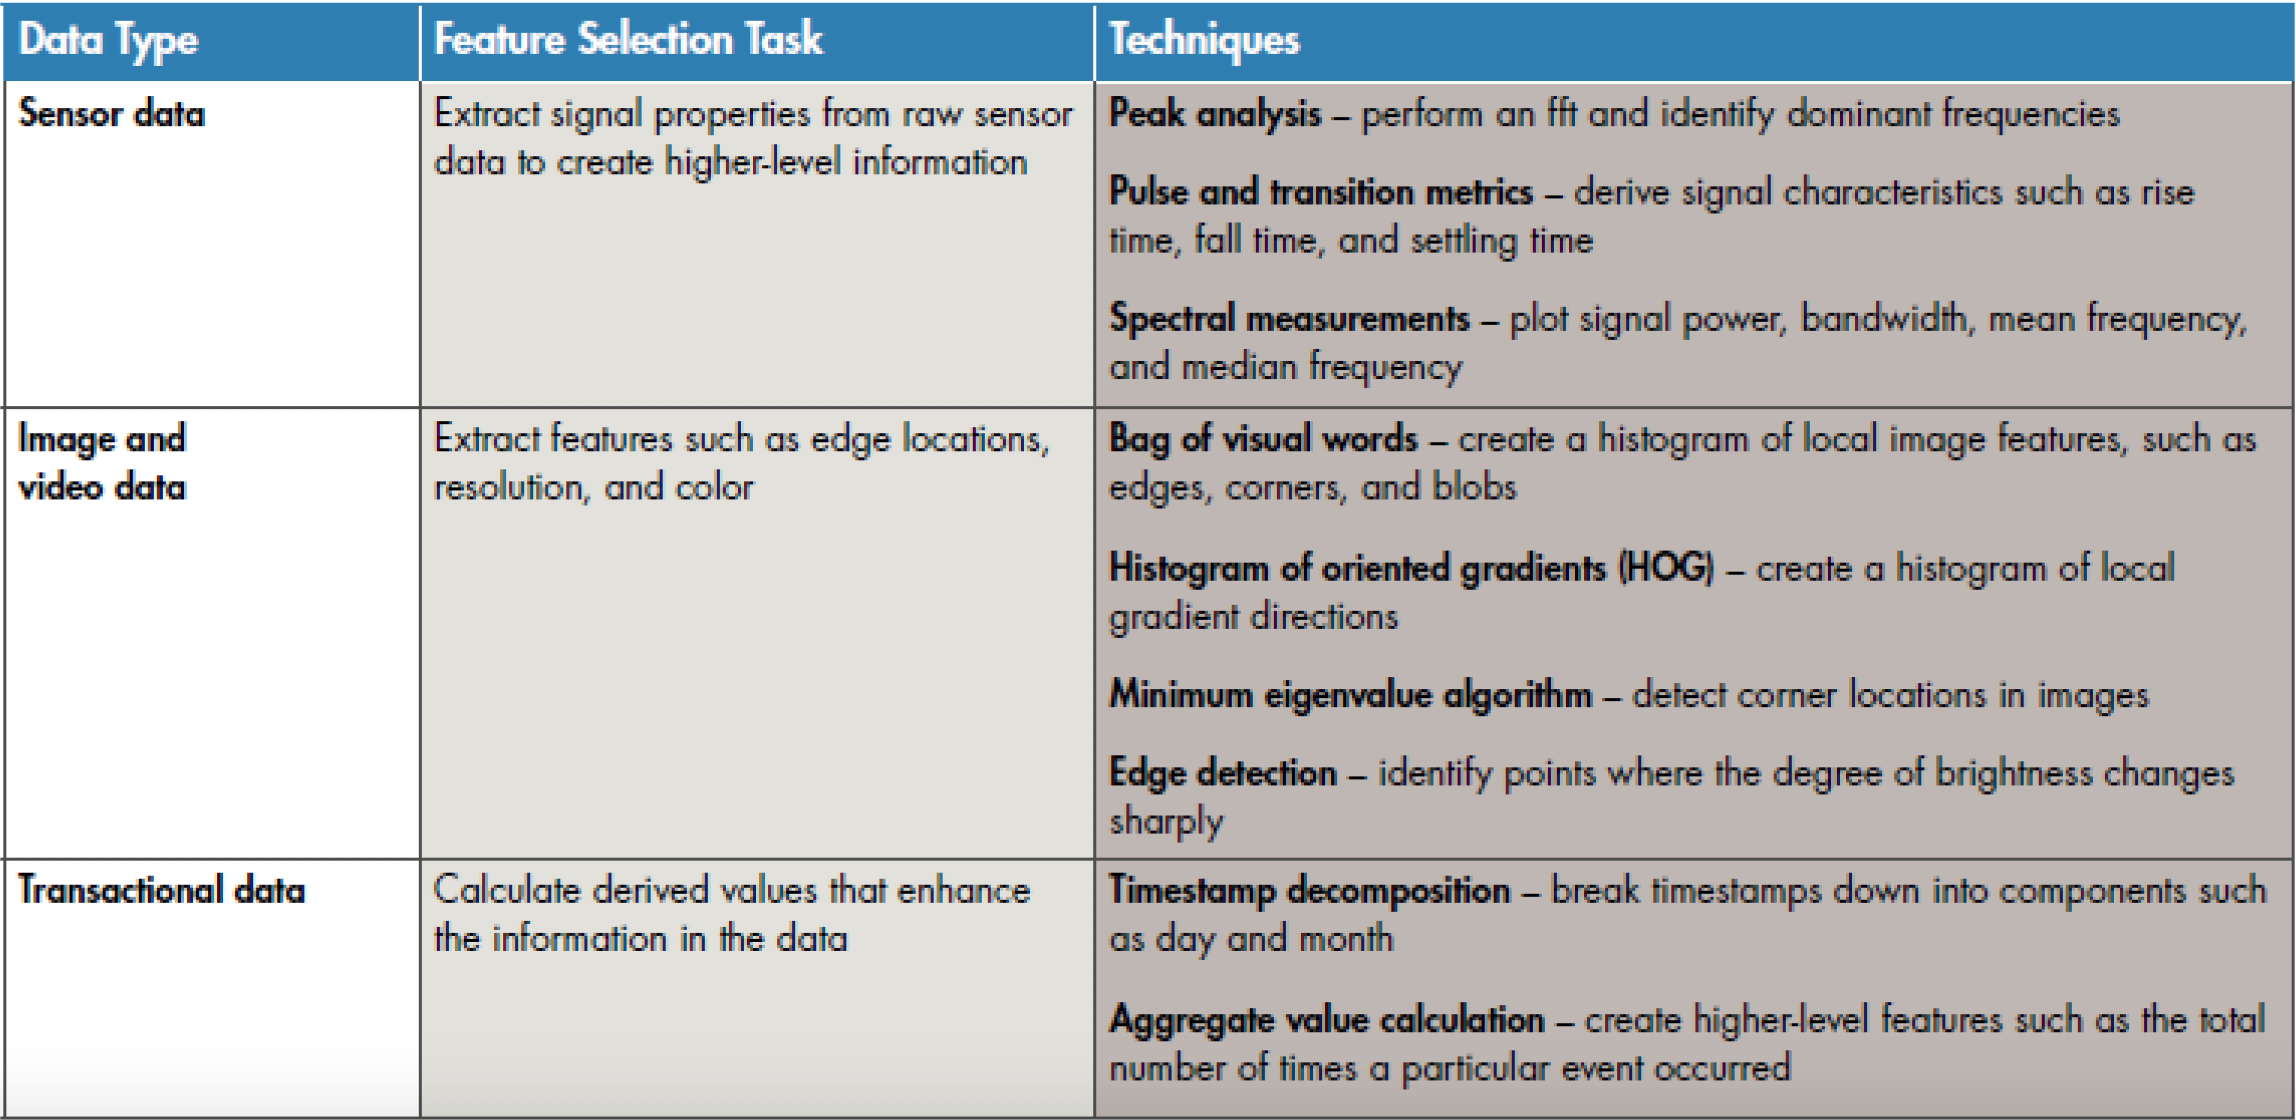
\includegraphics[width=.9\textwidth]{img/sw09/step_03.png}
				\caption{Common techniques used to derive features from data set}
			\end{figure}
			
			\subsubsection{Step 4: Build and Train the Model}
			
			When building a model, it's a good idea to start with something simple;
			It will be faster to run and easier to interpret.
			We start with a basic decision tree.
			
			\begin{figure}[htb!]
				\centering
				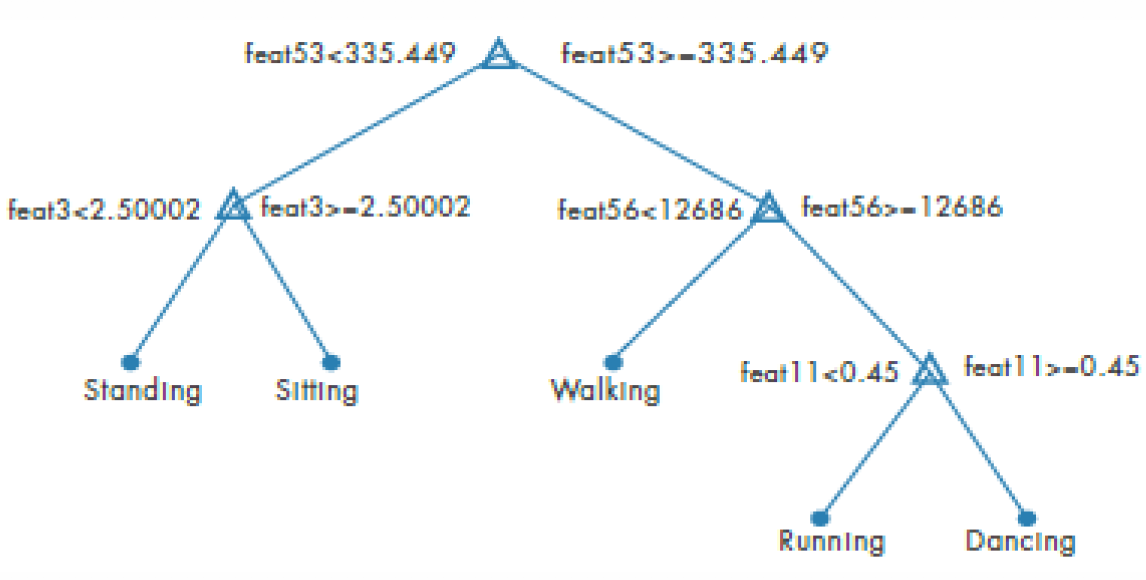
\includegraphics[width=.5\textwidth]{img/sw09/step4_tree.png}
			\end{figure}
		\noindent
			To see how well it performs, we plot the confusion matrix:
		
			\begin{figure}[htb!]
				\centering
				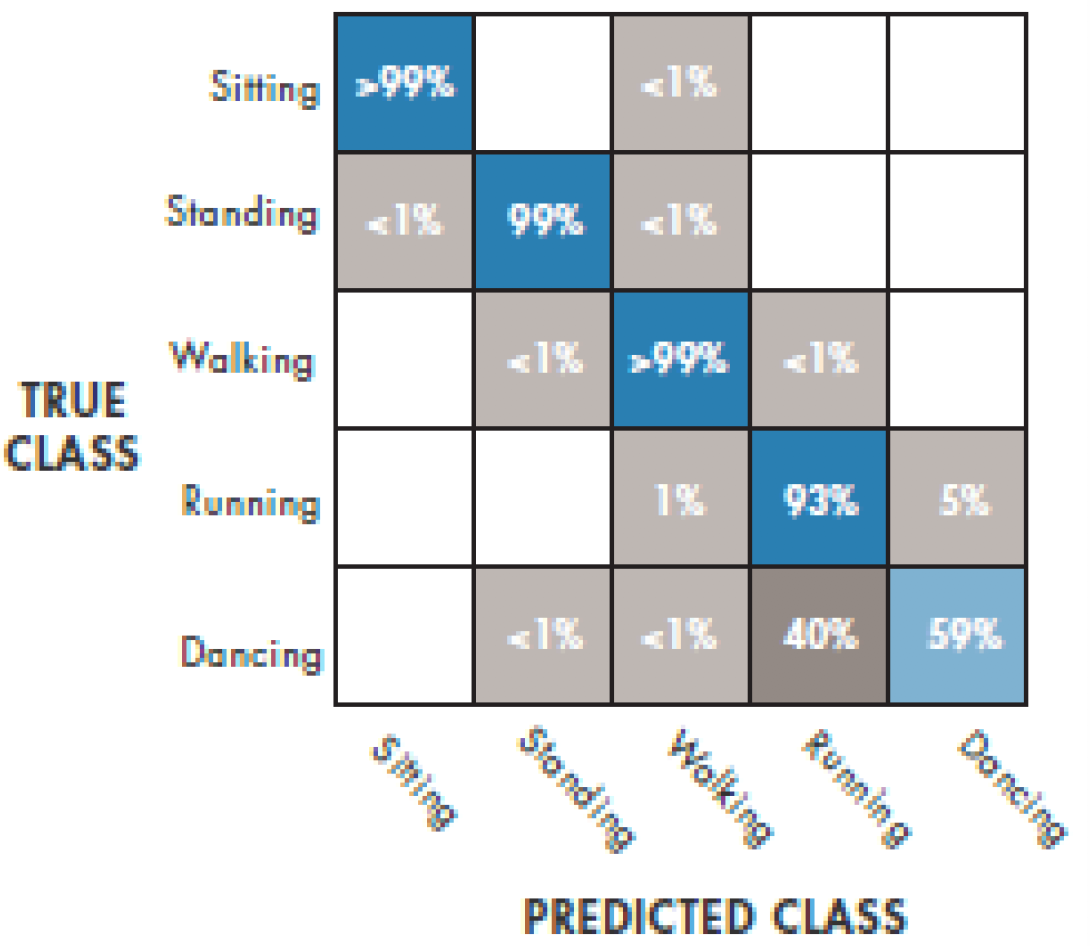
\includegraphics[width=.5\textwidth]{img/sw09/step4_matrix.png}
			\end{figure}
		\noindent
			It gives us a 94.1\% correct classification rate on train.
			Anyway, it also shows that our model is clearly having trouble distiguishing between dancing and running.
			Maybe a decision tree doesn't work for this type of data.
			Then, we will try a few different algorithms.
			
			\newpage
			
			K-nearest neighbors (KNN), a simple algorithm that compares new points to the training data and returns the most frequent class of the "K" nearest points.
			That gives us 98\% accuracy compared to 94.1\% for the simple decision tree and a better confusion matrix.
			
			\begin{figure}[htb!]
				\centering
				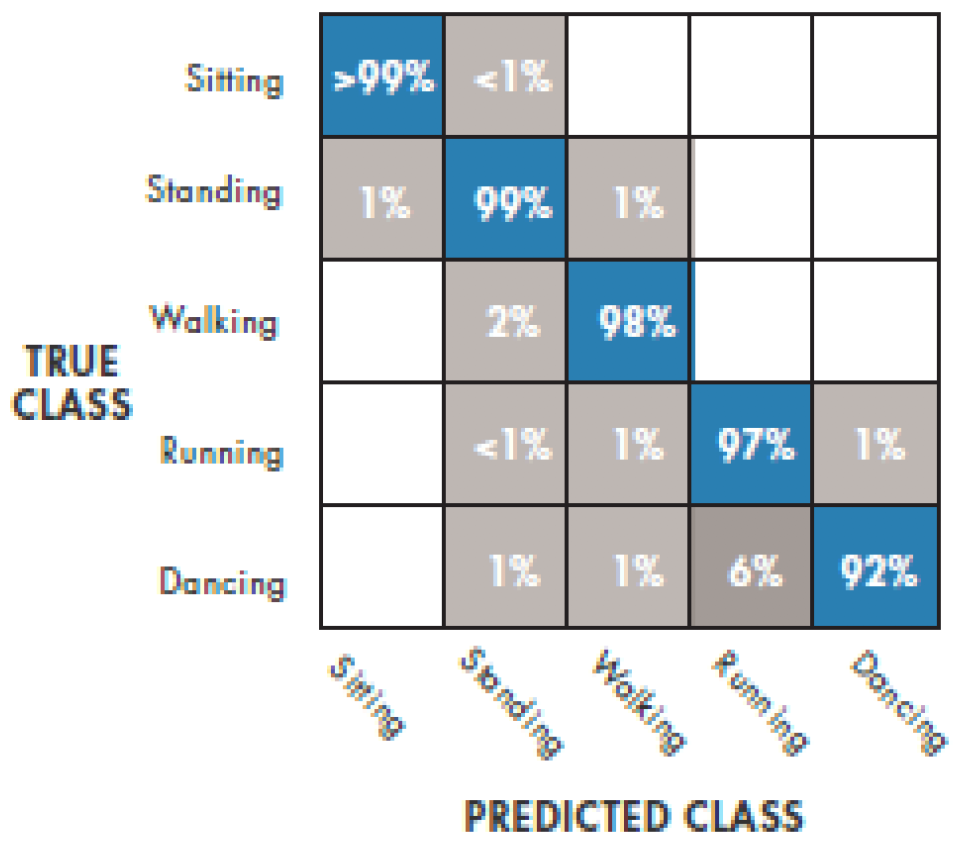
\includegraphics[width=.45\textwidth]{img/sw09/step4_knn.png}
			\end{figure}
			
			However, KNNs take a considerable amount of memory to run, since they require all training data to make a prediction.
			We try a linear discriminant model, but that doesn't improve the results.
			Finally, we try a multi-class support vector machine (SVM).
			The SVM does very well - we now get 99\% accuracy.
			
			\begin{figure}[htb!]
				\centering
				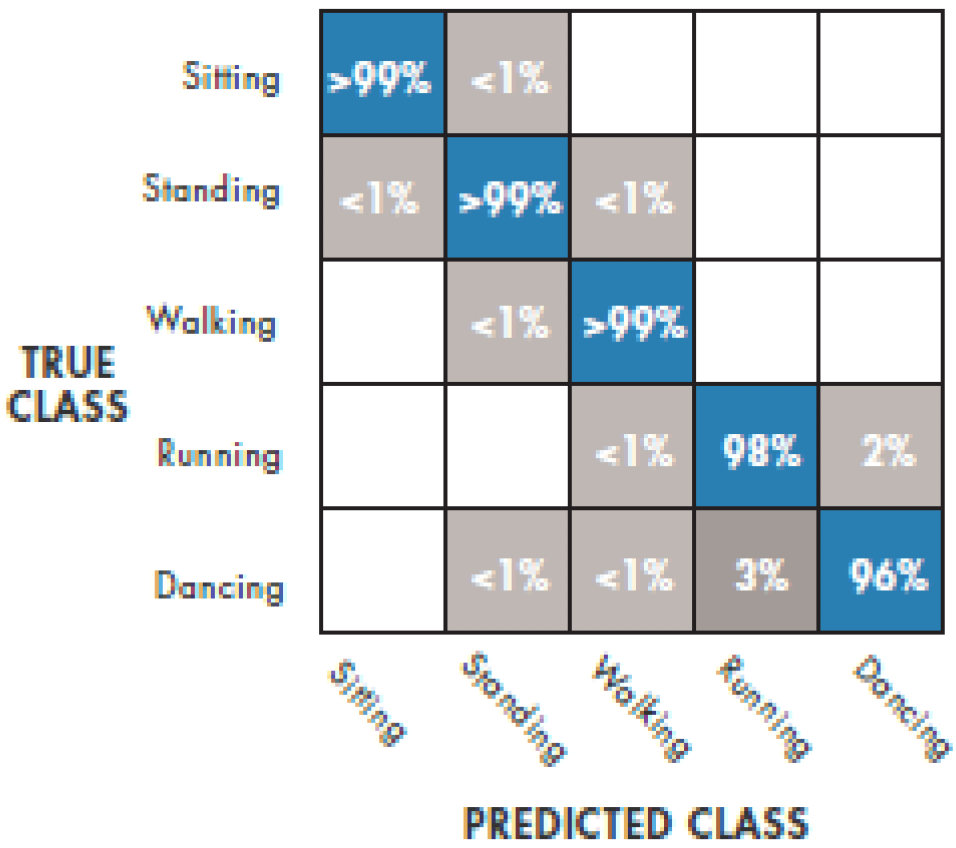
\includegraphics[width=.45\textwidth]{img/sw09/step4_svm.png}
			\end{figure}
		
			We achieved our goal by iterating on the model and trying different algorithms.
			If our classifier still couldn't reliably differentiate between dancing and running, we'd look into ways to improve the model.
			
			\newpage
				
			\subsubsection{Step 5: Improve the model}
			
			Improving a model can take two different directions:
			make the model simpler (simplify) or add complexity. \\
		\noindent
			First, we look for opportunities to reduce the number of features.
			Popular feature reduction techniques include:
			
			\begin{itemize}
				\item \textbf{Correlation matrix} - shows the relationship between variables, so that variables (or features), that are not highly correlated with the output, can be removed.
				\item \textbf{Principal component analysis (PCA)} - eliminates redundancy by finding a combination of features that captures key distinctions between the original features and brings out strong patterns in the dataset.
				\item \textbf{Sequential feature reduction} - reduces features iteratively on the model until there is no improvement in performance.
			\end{itemize}
		\noindent
			Next, we look at way to reduce the model itself.
			We can do this by:
				\begin{itemize}
					\item Pruning branches from a decision tree
					\item Removing learners from an ensemble
				\end{itemize}
		\noindent
			The other approach is to add Complexity:
			\begin{itemize}
				\item If our model can't differentiate dancing from running because it is over-generalizing, then we need to find ways to make it more fine-tuned.
			\end{itemize}
			To do this, we can either:
			\begin{itemize}
				\item \textbf{Use model combination} — merge multiple simpler models into a larger model that is better able to represent the trends in the data than any of the simpler models could on their own.
				\item \textbf{Add more data sources} — look at the gyroscope data as well as the accelerometer data.
					The gyroscope records the orientation of the cell phone during activity.
					This data might provide unique signatures for the different activities;
					e.g. there might be a combination of acceleration and rotation that's unique for running.
			\end{itemize}
			Once we've adjusted the model, we validate its performance on the test data that we set aside during preprocessing.
			If the model can reliably classify activities on the test data, we're ready to move it to the phone and start tracking.
		
		\subsection{How to choose the right model (ML view)}
		
		\begin{figure}[htb!]
			\centering
			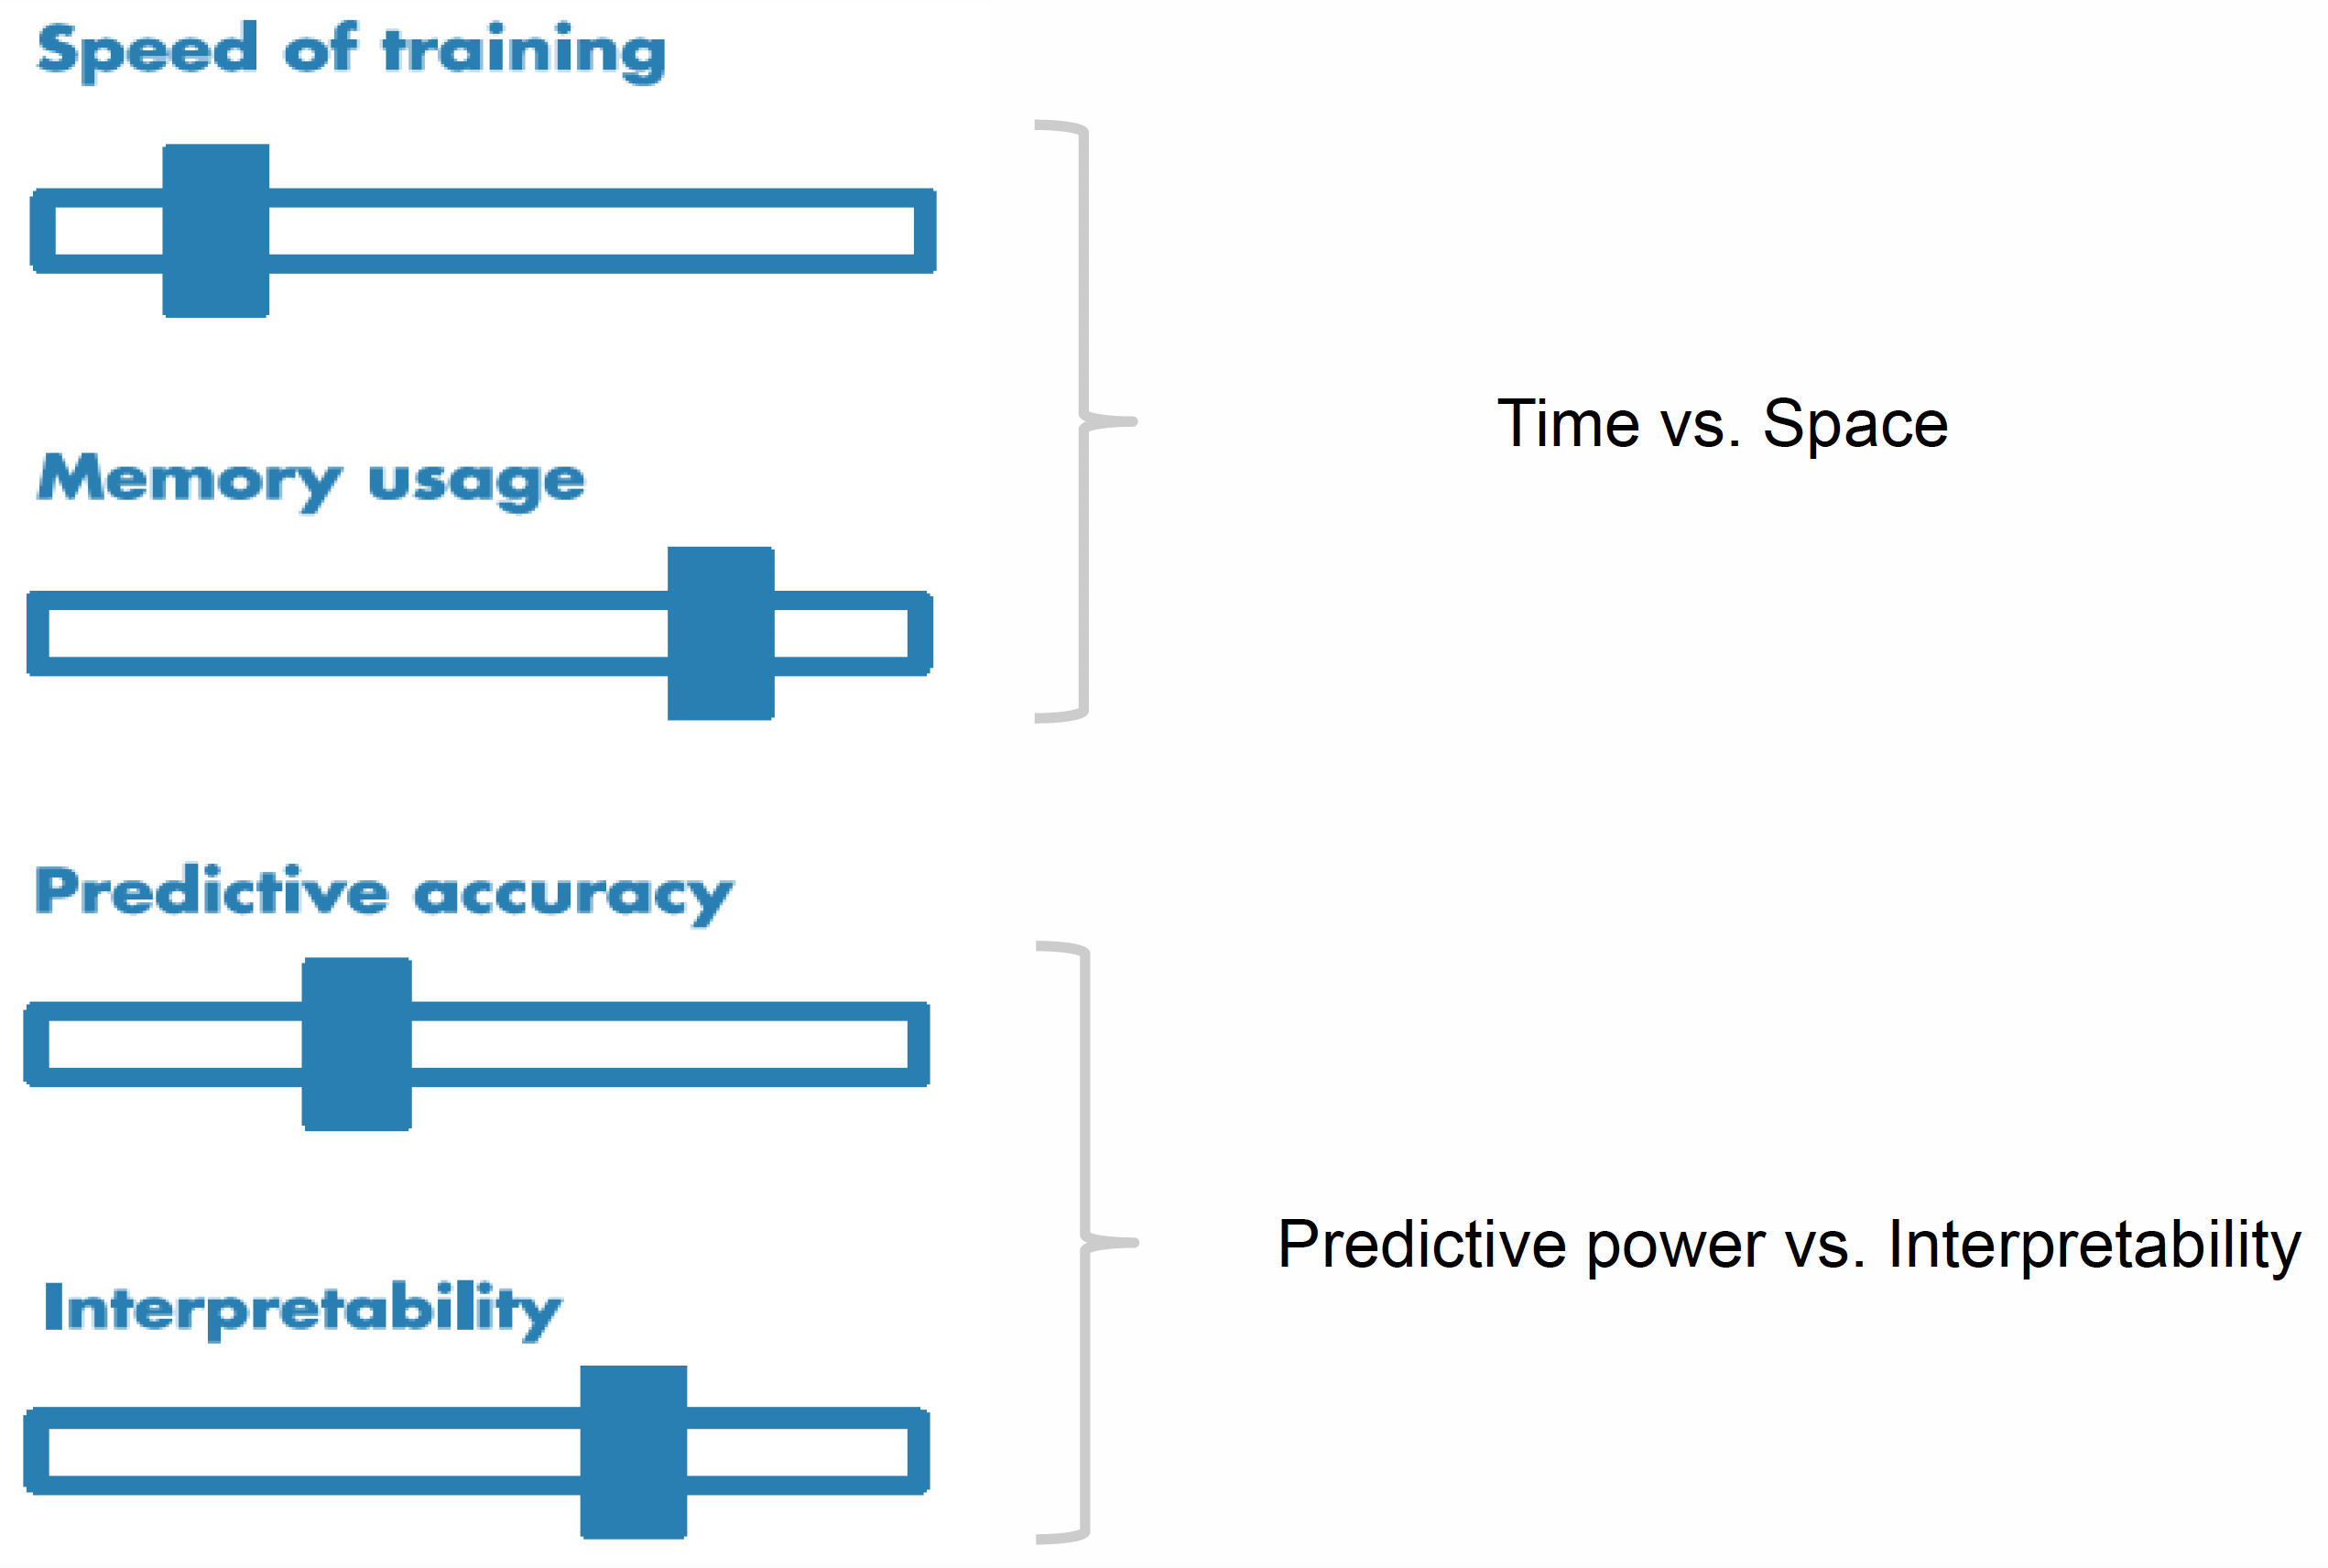
\includegraphics[width=\textwidth]{img/sw09/right_model.png}
		\end{figure}
	
	\newpage
	
	\section{Ethics in Data Science}
	
		\subsection{Data Ethics}
		
		\begin{itemize}
			\item Data ethics is an emerging branch of applied ethics.
			\item It describes the value judgements and approaches we make when generating, analysing and disseminating data.
			\item This includes:
				\begin{itemize}
					\item a sound knowledge of data protection law and other relevant legislation
					\item the appropriate use of new technologies
				\end{itemize}
			\item UK Data Ethics Framework (\href{https://assets.publishing.service.gov.uk/government/uploads/system/uploads/attachment_data/file/737137/Data_Ethics_Framework.pdf}{\textit{\underline{Link}}})
		\end{itemize}
	
		\begin{figure}[htb!]
			\centering
			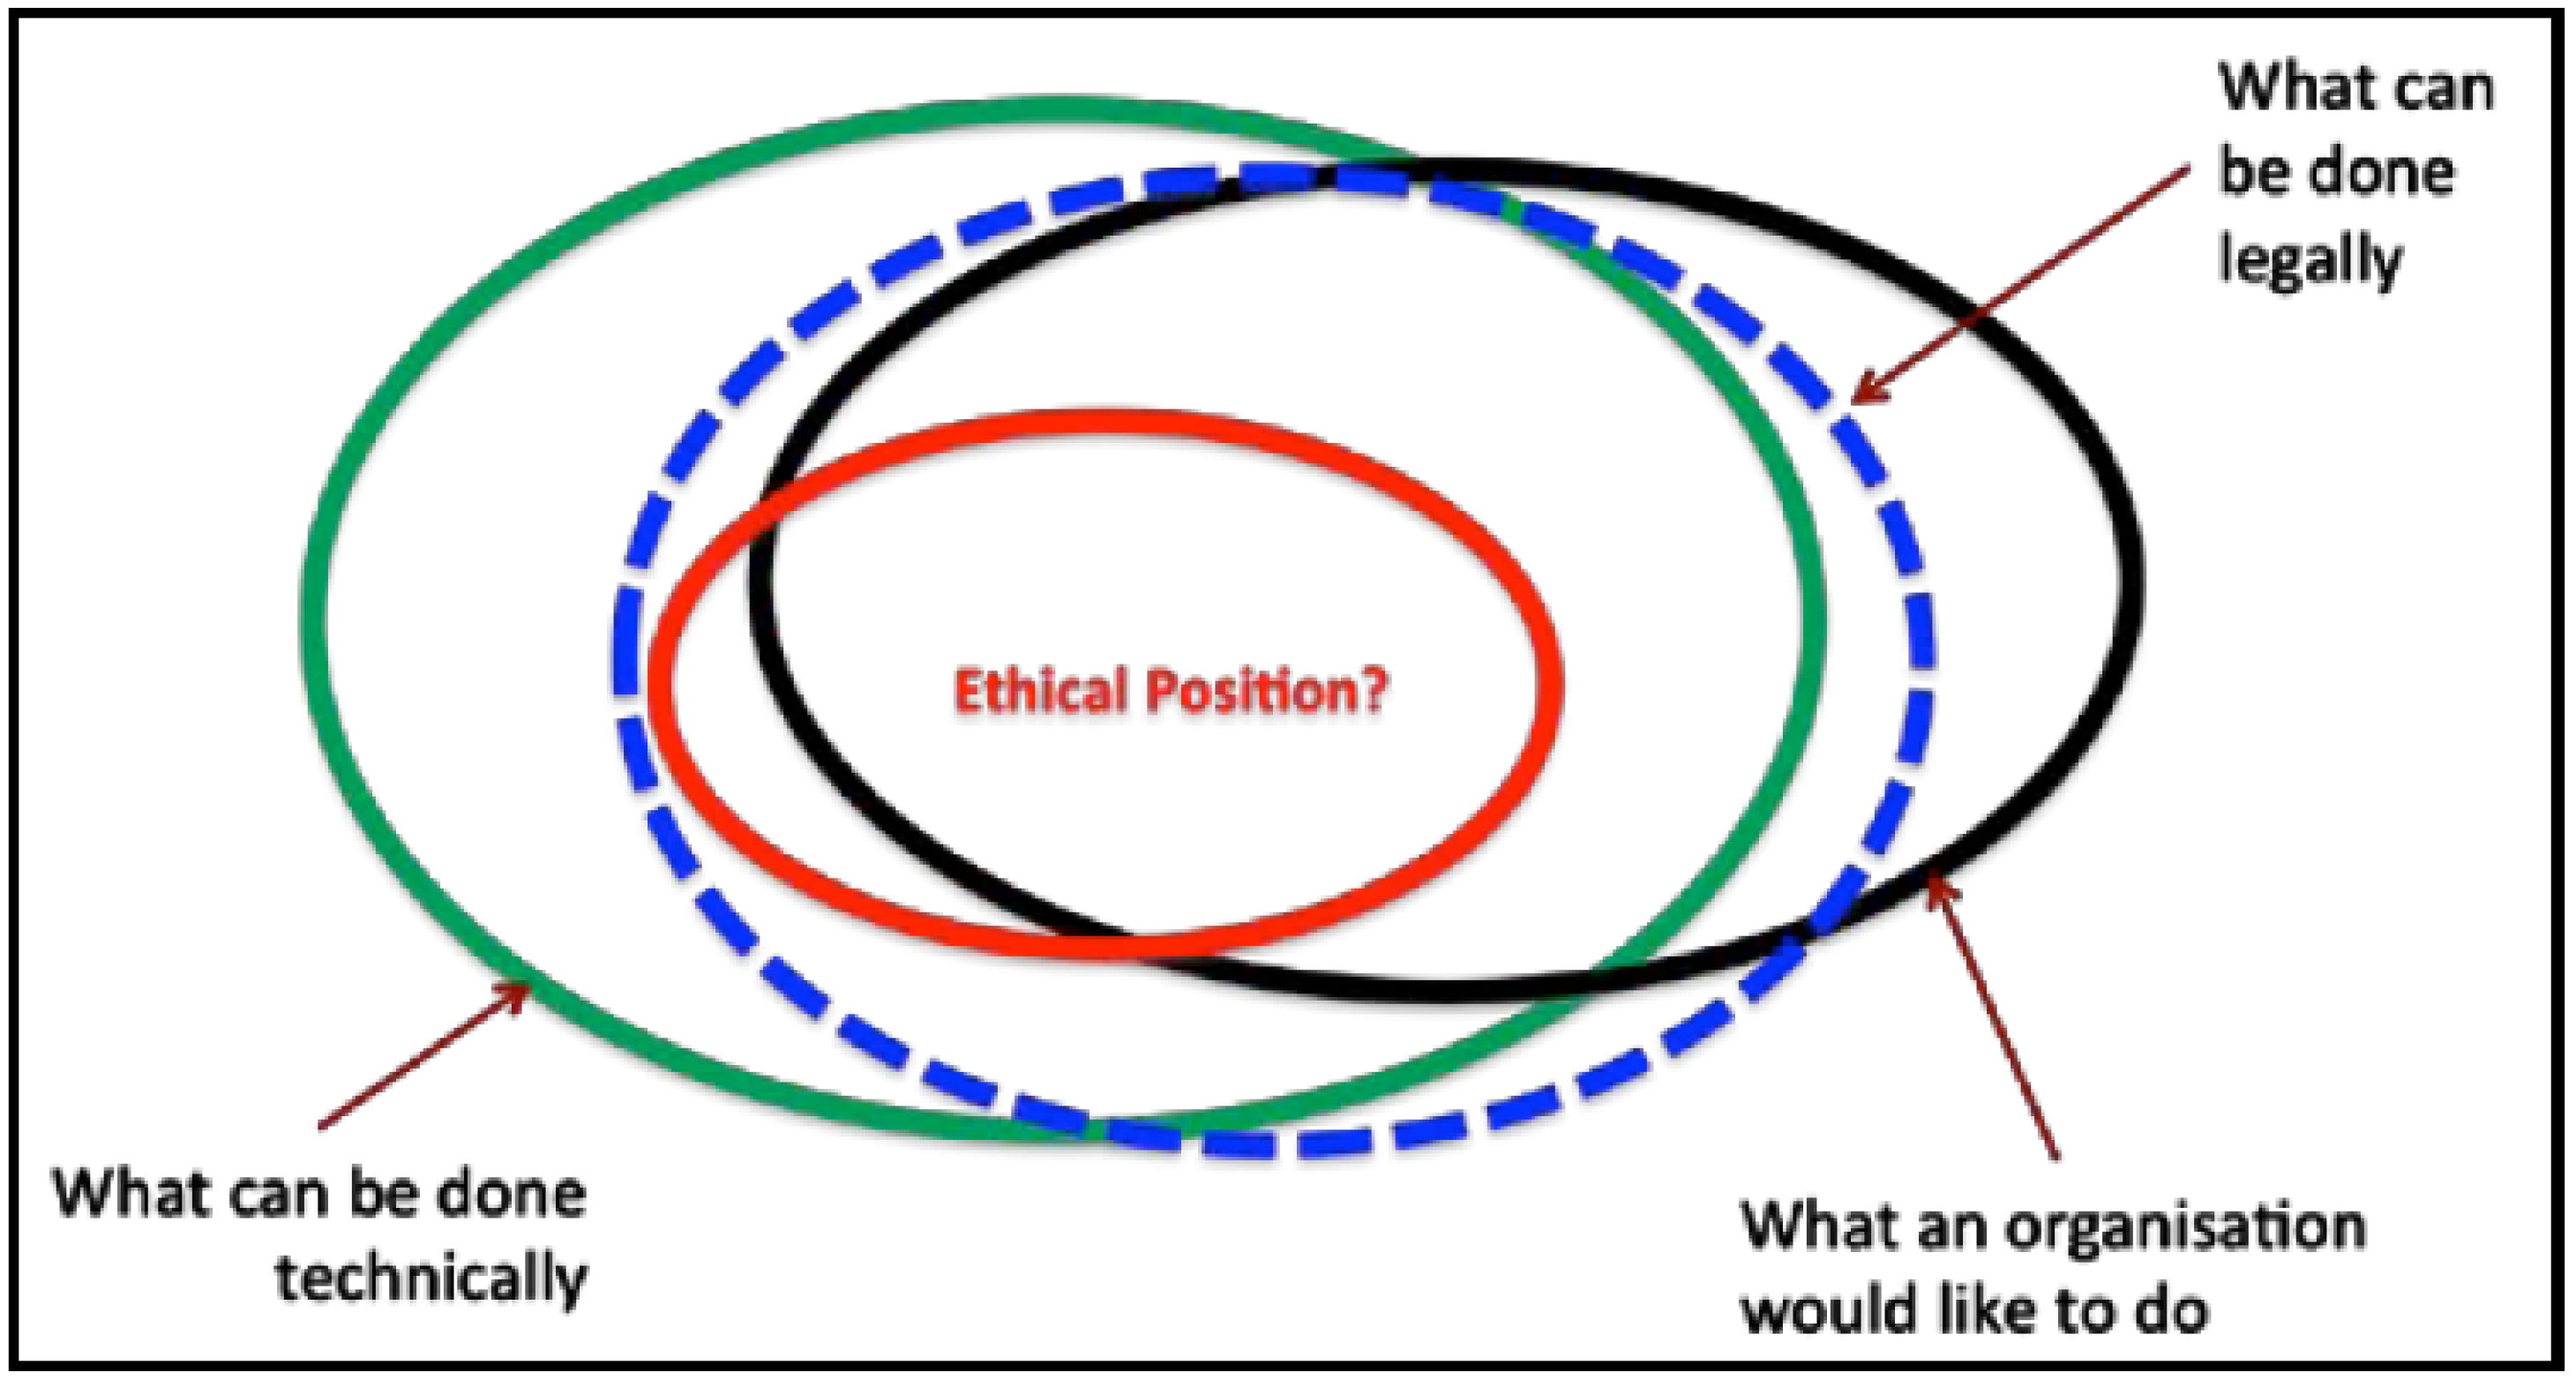
\includegraphics[width=.5\textwidth]{img/sw11/ethical_position.png}
		\end{figure}
	
		\subsection{Big Data Analytics and Data Science}
	
		\begin{itemize}
			\item Some of the distinctive aspects of big data analytics are:
				\begin{itemize}
					\item the use of algorithms
					\item the opacity of the processing
					\item the tendency to collect "all the data"
					\item the re-purposing of data
					\item the use of new types of data
				\end{itemize}
			\item Types of data:
				\begin{itemize}
					\item \textbf{Provided data} is consciously given by individuals, e.g. when filling in an online form
					\item \textbf{Observed data} is recorded automatically, e.g. by online cookies or sensors or CCTV linked to facial recognition
					\item \textbf{Derived data} is produced from other data in a relatively simple and straightforward fashion, e.g. calculating customer profitability
				\end{itemize}
		\end{itemize}
	
		\subsection{Possible problems with data science}
		
		\begin{itemize}
			\item Some types of big data analytics, such as profiling, can have intrusive effects on individuals
				\begin{itemize}
					\item it may use personal data to make decisions affecting individuals
					\item e.g. credit limits, but also promotions ("people analytics")
				\end{itemize}
			\item Organisations need to consider whether the use of personal data in big data applications is within people's reasonable expectations
			\item The complexity of the methods of big data analysis, such as machine learning, can make it difficult for organizations to be transparent about the processing of personal data.
		\end{itemize}
	
		\newpage
	
		\subsection{Ethical concerns about personal data}
		
		\begin{itemize}
			\item \textbf{Surveillance}\\
				A 2013 study by the Wellcome Trust, consisting of focus groups and telephone interviews, found there to be a \textit{"widespread wariness" about being spied on} by the government, corporations and criminals.
			\item \textbf{Discrimination}\\
				The same study revealed concerns about \textit{possible discrimination against people} based on medical data, for instance where such data is shared with employers who might make discriminatory decisions about people because of mental health issues.
			\item \textbf{Consent}\\
				An online survey conducted by Demos in 2012 found that people's top concern for personal data use was about \textit{companies using it without their consent}.
			\item \textbf{Data sharing}\\
				The Institute for Insight in the Public Services conducted a telephone survey in 2008 which revealed that while people are generally happy for their personal data to be held by one organisation, they are concerned when it is shared with others.
				These concerns centered on \textit{loss of control over personal data} and fears that \textit{errors in the data would be perpetuated through sharing}.
		\end{itemize}
	
		\subsection{Conditions for processing personal data}
		
		\begin{enumerate}
			\item \textbf{Consent} must be a freely given, specific and informed indication that subjects agree to the data processing.
			\item Data processing must be necessary for the \textbf{legitimate interests of the organization} collecting the data.
			\item Data processing must be \textbf{necessary for the performance of a contract} to which the data subject is a party.
		\end{enumerate}
	\vspace{1em}
	\noindent
		Big data analysis carried out in the public sector may be legitimized by other conditions, for instance where processing is necessary for the exercise of functions of a government department.
		
		\subsection{Purpose Limitation}
		
		\begin{itemize}
			\item The purpose limitation principle does not necessarily create a barrier for big data analytics, but it means an \textbf{assessment of compatibility} of processing purposes must be done.
				\begin{itemize}
					\item First, the \textbf{purpose} for which the data is collected must be specified and lawful.
					\item Second, if the data is further processed for any other purpose, it \textbf{must not be incompatible with the original purpose}.
					\item If an organization is buying personal data from elsewhere for big data analytics, it needs to \textbf{practice} \href{https://en.wikipedia.org/wiki/Due_diligence}{\textit{\textbf{due diligence}}}.
						It will need to assess whether the new processing is incompatible with the original purpose for which the data was collected.
				\end{itemize}
			\item \textbf{Fairness} is a key factor in determining whether big data analysis is incompatible with the original processing purpose. 
		\end{itemize}
	
		\subsection{Data Minimization: Collection \& Retention}
		
		\begin{itemize}
			\item Big data analytics can result in the collection of personal data that is excessive for the processing purpose.
			\item Organizations may be encouraged to retain personal data for longer than necessary because big data applications are capable of analyzing large volumes of data.
		\end{itemize}
	
		\newpage
	
		\subsection{Accuracy}
		
		\begin{itemize}
			\item There are implications regarding the \textbf{accuracy} of personal data at all stages of a big data project: collection analysis and application.
				\begin{itemize}
					\item Personal data must be accurate and, where necessary, kept up to date
				\end{itemize}
			\item Results of data analysis may not be \textbf{representative} of the population as a whole.
			\item \textbf{Hidden biases} in data sets can lead to inaccurate predictions about individuals.
		\end{itemize}
	
		\subsection{Rights of Individuals}
		
		\begin{itemize}
			\item The vast quantities of data used in big data analytics may make it more difficult for organisations to comply with the \textbf{right of access to personal data}.
			\item People have the right to be told:
				\begin{itemize}
					\item What personal data about them is being processed.
					\item The purposes for which it is being processed.
					\item Who it may be disclosed to.
					\item They have the right to receive a copy of the information that constitutes their personal data, as well as information about its sources.
				\end{itemize}
			\item Organisations will need to have appropriate processes in place to deal with the GDPR's extension of \textbf{rights regarding decisions based on automated processing}.
			\item People have the \textbf{right not to be subject to a decision based solely on automated processing}, including profiling, if it "significantly affects" them, such as automated decisions made on online credit applications, VISA emission or e-recruitement.
		\end{itemize}
	
		\subsection{Security}
		
		\begin{itemize}
			\item There are several \textbf{information security risks} specific to big data analytics.
				\begin{itemize}
					\item E.g. the high level of replication in big data storage and the frequency of outsourcing the analytics increase the risk of breaches, data leakages and degradation; also, the creation of links between the different datasets could increase the impact of breaches and leakages.
				\end{itemize}
			\item Organisations need to recognize these new risks and put in place appropriate security measures. (\href{https://ico.org.uk/media/for-organisations/documents/1540/cloud_computing_guidance_for_organisations.pdf}{Link for Cloud Computing})
		\end{itemize}
	
		\subsection{Accountability and Governance}
		
		\begin{itemize}
			\item \textbf{Accountability} is increasingly important for big data analytics and will become an explicit requirement under the GDPR.
				\begin{itemize}
					\item Records of processing activities must be maintained when processing personal data that could result in a risk to individuals' rights and freedoms.
				\end{itemize}
			\item Big data organisations may need to \textbf{make changes to their reporting structures}, internal record keeping and resource allocation.
			\item Machine learning algorithms have the potential to make decisions that are \textbf{discriminatory, erroneous and unjustified}.
			\item \textbf{Data quality} is a key issue for those with information governance responsibilities in a big data context.
		\end{itemize}
	
		\subsection{Data Controllers \& Data Processors}
		
		\begin{itemize}
			\item Big data analytics can make it difficult to distinguish between \textit{data controllers} and \textit{data processors}.
			\item A data controller has \textbf{overall control over the processing of personal data} - it determines the purposes and manner of the processing, either on its own, jointly or in common with another data controller.
			\item A data processor does not have such control - it merely \textbf{processes personal data on a data controller's behalf}.
			\item Organizations outsourcing analytics to companies specializing in AI and machine learning need to consider carefully who has control over the processing of any personal data.
		\end{itemize}
	
		\newpage
		
		\subsection{Key Recommendations}
		
			\subsubsection{Anonymization}
			
			\begin{itemize}
				\item Carefully \textbf{consider} whether the big data analytics to be undertaken actually requires the processing of personal data.
				\item Ofthen, this will not be the case; in such circumstances, organizations should use appropriate techniques to \textbf{anonymize} the personal data in their dataset(s) before analysis.
			\end{itemize}
		
			\subsubsection{Privacy Notices}
			
			\begin{itemize}
				\item Be \textbf{transparent} about their processing of personal data by using a combination of innovative approaches in order to provide meaningful privacy notices at appropriate stages throughout a big data project.
				\item This may include the use of icons, just-in-time notifications and layered privacy notices.
				\item The processing of personal data cannot be considered \textbf{fair} unless the data subject is given some basic information about it, including the data controller's identity, the purpose of the processing and any other information necessary.
				\item Ticking a box to say "I have read and agreed to the terms and conditions" has been described as \textbf{"the biggest lie on the web"}.
			\end{itemize}
		
			\subsubsection{Privacy Impact Assessment}
			
			\begin{itemize}
				\item Embed a \textbf{privacy impact assessment framework} into the big data processing activities to help identify privacy risks and assess necessity and proportionality of a given project.
				\item The privacy impact assessment should involve \textbf{input from all relevant parties} including data analysts, compliance officers, board members and the public.
			\end{itemize}
	
			\subsubsection{Privacy by Design}
			
			\begin{itemize}
				\item Adopt a privacy by design approach in the development and application of their big data analytics.
				\item This should include implementing \textbf{technical and organizational measures} to address matters including \textit{data security, data minimization and data segregation}.
			\end{itemize}
		
			\subsubsection{Ethical Approaches}
			
			\begin{itemize}
				\item Develop ethical principles to help reinforce key data protection principles.
				\item Employees in smaller orgaisations should use these \textbf{principles as a reference point} when working on big data projects.
					Conversely, larger organizations (e.g. IBM, Accenture are doing it) should create ethics boards to help scrutinise projects and assess complex issues arising from big data analytics.
			\end{itemize}
		
			\subsubsection{Algorithmic Transparency}
			
			\begin{itemize}
				\item Implement innovative techniques to develop \textbf{auditable} machine learning algorithms \\
					($\rightarrow$ explainable AI)
				\item Internal and external audits should be undertaken with a view to \textbf{explaining the rationale behind algorithmic decisions} and checking for bias, discrimination and errors.
			\end{itemize}
				
\end{document}
